%#!platex ./report.tex

%
% $B%3%s%@%/%?%s%9$K$D$$$F!"$J$<(BCaT$B!"(BKa$B$rMQ$$$k$N$+$r=q$$$F$*$/(B
%

%
% $B@h9T8&5f$NI>2A<jK!$r$h$/8@5Z$7$F$$$k$N$G!"$3$3$K=q$$$F$*$$$?$[$&$,$$$$$+$b(B
%

\chapter{$B8&5f<jK!!&86M}(B}
 \section{$B8&5f<jK!$N35MW(B}
   $BK\8&5f$N<jK!$N35N,$O0J2<$N$h$&$J$b$N$G$"$k(B.
   \begin{enumerate}
     \item $BC10l$N?@7P:YK&$N5!G=$r(B1$B$D7h$a$k(B
     \item $B$=$N5!G=$r$&$^$/<B8=$9$k?@7P:YK&$N7ABV$H%3%s%@%/%?%s%9J,I[$r(B
       $B0dEA%"%k%4%j%:%`$rMQ$$$FC5:w$9$k(B
   \end{enumerate}
   $BK\8&5f$N<jK!$O<g$K(BTorben-Nielsen et al. $B$r;29M$K$7$F$$$k(B\cite{torben2009systematic}.
   $B?@7P:YK&$N7ABV$H5!G=$N4X78@-$rC5$k%"%W%m!<%A$H$7$F(B, 
   $B?@7P:YK&$N7ABV$+$i$=$N5!G=$r?dDj$9$k$N$G$O$J$/(B, $B@h$K5!G=$r@_Dj$7$=$N5!G=$r(B
   $B<B8=$9$k7ABV$rC5$9$H$$$&<jK!$G$"$k(B. 
 \section{$B?@7P:YK&$N5!G=(B}
   $BK\8&5f$G?@7P:YK&$K@_Dj$9$k5!G=$O(B, $B<y>uFM5/>e$N0[$J$k(B2$B$D$NIt0L$K$"$k;~4V(B
   $B:9(B${\Delta}t[{\rm ms}]$$B$r$b$C$FF~NO;I7c$rM?$($?>l9g(B, $BF~NO$N=g=x$K$h$C$F:YK&BN$G$N(B
   $BC&J,6KNL$,JQ2=$9$k5!G=(B(input-order detection)$B$G$"$k(B. $B$h$j6qBNE*$K$O(B
   $B<!$N$h$&$J5!G=$G$"$k(B. \\
   $B$"$k?@7P:YK&$,6u4V>e$KJ,N%$7$?(B2$B$D$NNN0h$K<y>uFM5/$r?-$P$7(B, $B$=$l$>$l$N(B
   $BNN0hCf$K$$$/$D$+$N%7%J%W%9$r7A@.$7$F$$$k$H$9$k(B. $B2>$K$3(B
   $B$N(B2$B$D$NNN0h$r(BBlue$B%7%J%W%F%#%C%/%>!<%s(B, Red$B%7%J%W%F%#%C%/%>!<(B
   $B%s$H$9$k(B. Blue$B%7%J%W%F%#%C%/%>!<%s$K7A@.$5$l$?%7%J%W%9$r(BBlue$B%7%J%W%9(B,
   Red$B%7%J%W%F%#%C%/%>!<%s$K$D$$$F$bF1MM$K(BRed$B%7%J%W%9$H$9$k(B. 
   $B$3$N?@7P:YK&$K$*$$$F(B, $B0lJ}$N%7%J%W%F%#%C%/%>!<%s$NA4$F$N%7%J%W%9$r;~9o(B$t$$B$G3h@-2=(B
   $B$5$;(B, $B$=$N(B${\Delta}t[{\rm ms}]$$B8e$KB>J}$N%7%J%W%F%#%C%/%>!<%s$N%7%J%W%9$r3h@-2=$5$;$k(B.
   $B$=$N:]$K:YK&BN$G4QB,$5$l$k:GBg$NKlEE0L>e>:NL$r(B$R$$B$H$9$k(B. Blue$B%7%J%W%F%#%C%/%>!<%s$N(B
   $B%7%J%W%9$,@h$K3h@-2=$9$k>l9g$N(B$R$$B$r(B$R_{B{\to}R}$$B$H$7(B, Red$B%7%J%W%F%#%C%/%>!<%s$N%7%J%W%9$,(B
   $B@h$K3h@-2=$9$k>l9g$N(B$R$$B$r(B$R_{R{\to}B}$$B$H$9$k(B. $B$3$N$H$-(Binput-order detection$B$N(B
   $B5!G=@-(B($F$)$B$O0J2<$N<0$K$h$C$FDjNLE*$KI>2A$9$k$3$H$,$G$-$k(B. 

   \begin{equation}
     F = \frac{R_{B{\to}R}}{R_{R{\to}B}}
     \label{F}
   \end{equation}

   $B$^$?K\8&5f$G$OBg$-$$(B$F$$B$NCM$r<($9?@7P:YK&$K$D$$$F(B, $B5!G=@-$N9b$$?@7P:YK&$G$"$k$HDj5A$9$k(B. 
   $B0J2<$N?^(B\ref{sample}$B$K?@7P:YK&$H(B, $B%7%J%W%F%#%C%/%>!<%s$rNc<($9$k(B. $B?^(B\ref{Neuron}$B$N(B
   $B>eIt$K$"$k@V$$E@$O(BRed$B%7%J%W%9(B, $B2<It$N@D$$E@$O(BBlue$B%7%J%W%9$rI=$7(B, $BCf1{$N(B
   $B5e$O:YK&BN$G$"$k(B.  $B?^(B\ref{synaptic-zone}$B$NCf1{$NNP$NE@$O:YK&BN$G$"$j(B,
   $B$3$N?^$O?@7P:YK&$H%7%J%W%F%#%C%/%>!<%s$H$N(B
   $B0LCV4X78$r?^<($7$F$$$k(B. $B?^(B\ref{input-order_detection}$B$O?^(B\ref{Neuron}$B$K<($5$l$k?@7P:YK&$K(B
   $BBP$7(B, ${\Delta}t = 15$[ms]$B$H$7$F%7%J%W%9F~NO$rM?$($?:]$N:YK&BN$G$NKlEE0LJQF0$r<($7$F$$$k(B. 
   $B?^(B\ref{input-order_detection}$B$N>l9g(B, $R_{B{\to}R} = 6.29$, $R_{R{\to}B} = 4.75$$B$h$j(B
   $F = 1.32$$B$G$"$k(B.
   
   \begin{figure}
     \centering
     \begin{subfigure}{0.3\columnwidth}
       \centering
       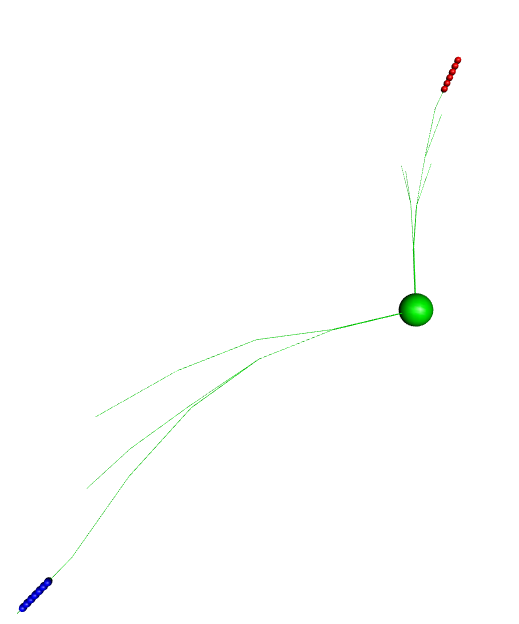
\includegraphics[width=\columnwidth]{./Images_Method/pass_neuron.png} 
       % $BGX7J$OGr$NJ}$,NI$5$=$&(B
       % rgl$B$N;0<!852hA|$O(Beps$B$K$7$J$$$[$&$,$h$$(B
       \caption{$B?@7P:YK&$NNc(B}
       \label{Neuron}
     \end{subfigure}
     \begin{subfigure}{0.2\columnwidth}
       \centering
       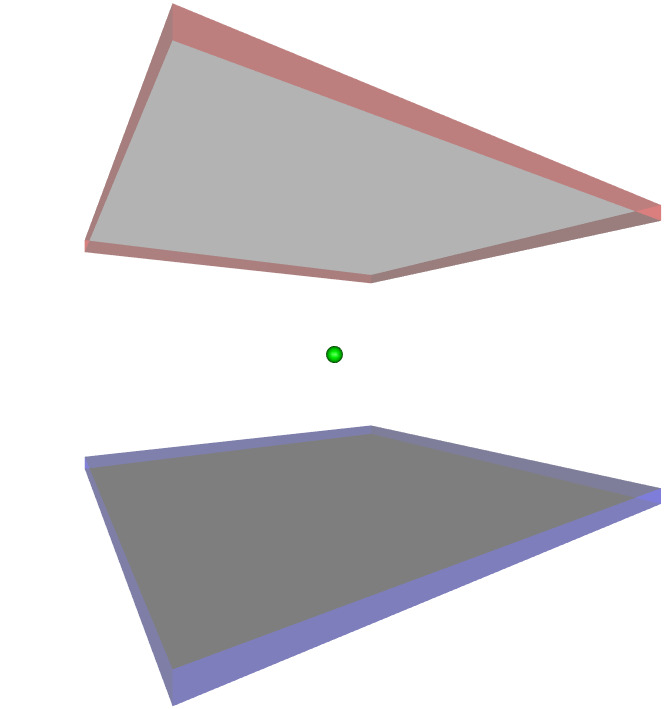
\includegraphics[width=\columnwidth]{./Images_Method/synaptic_zone.png}
       \caption{$B%7%J%W%F%#%C%/%>!<%s(B}
       \label{synaptic-zone}
     \end{subfigure}
     \begin{subfigure}{0.4\columnwidth}
       \centering
       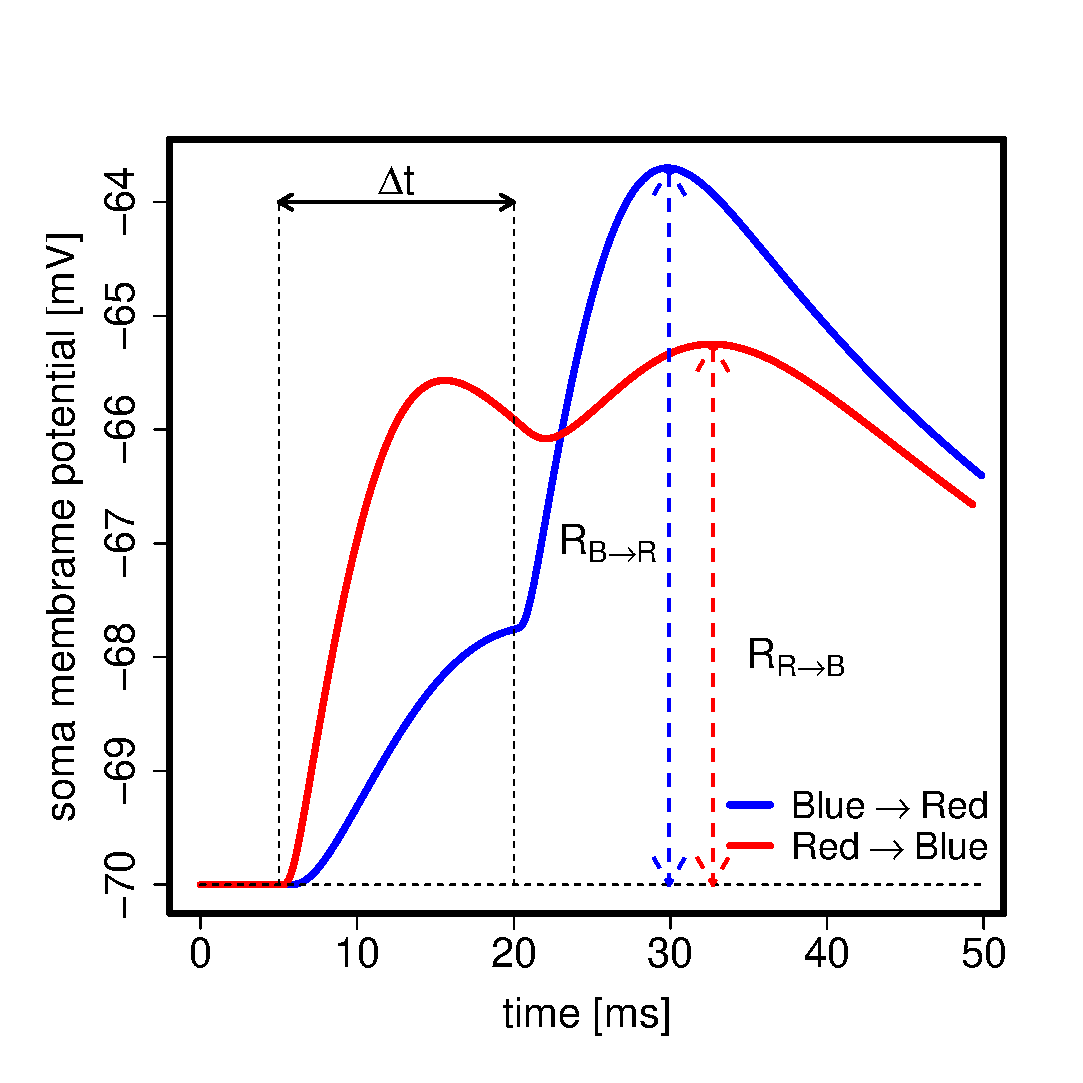
\includegraphics[width=\columnwidth]{./Images_Method/input_order_detection.eps} 
       \caption{input-order detection}
       \label{input-order_detection}
     \end{subfigure}
     \caption{$B:n@.$7$??@7P:YK&$H(Binput-order detection}
     \label{sample}
   \end{figure}

   %
   % input-order detection$B$K$D$$$F(B passive$B$N>l9g(BF$B$N:GBgCM$O(B2$B$H;W$o$l$k$H=q$$$F$*$/(B
%     \subsection{input-order detection$B$K$D$$$F(B}
%  Passive$B%b%G%k$rMQ$$$k$H(B, $BKlFC@-$,KlEE0L$K$h$C$FJQ2=$7$J$$$?$a:YK&BN$G$NKlEE0L>e>:$O(B
   %  $BF~NOEEN.$NC1=c$J2C;;$H$J$k(B. $B$D$^$j(Binput-order detection$B$N(B$F$$BCM$N:GBgCM$O(B2$B$K$J$k$H9M$($i$l$k(B.

   %$B$3$l$O7k2L$NJ}$K=q$/$Y$-$+(B?
   
   %% \subsection{Ka$B%3%s%@%/%?%s%9(B, CaT$B%3%s%@%/%?%s%9$N8z2L(B}
   %%   $B?@7P:YK&$K(BKa$B%3%s%@%/%?%s%9$rF3F~$9$k$H(B, $BKlEE0L$r2<$2$kF/$-$r$9$k(B. input-order detection
   %%   $B$G$O<g$K(BRed$B%7%J%W%0%k!<%W$+$i$NF~NO$,$3$N1F6A$r<u$1$k(B. $B$D$^$j(BRed$B%7%J%W%9%0%k!<%W$N(B
   %%   $BF~NO$K$h$k:YK&BN$G$NC&J,6K$,$h$j>.$5$/(B, $B8:?j$bAa$/$J$k(B.
   %%   CaT$B%3%s%@%/%?%s%9$rF3F~$7$?>l9g$O5U$KKlEE0L$r>e>:$5$;$kF/$-$r$9$k(B. input-order detection
   %%   $B$G$O(BBlue$B%7%J%W%9%0%k!<%W$,$3$N1F6A$r<u$1(B, $B:YK&BN$G$NC&J,6K$,$h$jBg$-$/8:?j$bCY$/$J$k(B. 
   
 \section{$B?@7P:YK&7ABV$N:n@.J}K!(B}
   $B4JC1$N$?$a?@7P:YK&$N7ABV$O:YK&BN$H(B2$BK\$N<y>uFM5/$+$i$J$k$H$9$k(B. $B$9$J$o$A(B,
   $B>e2<$N%7%J%W%F%#%C%/%>!<%s$K$N$S$k(B2$BK\$N<y>uFM5/$H(B, $BF~NO$r2C;;$9$k:YK&BN$G$"$k(B. 
   $B:YK&BN$N7ABV$O0lDj$NBg$-$5$N5e7A$G$"$k$H$9$k(B. 
   $B$h$C$F?@7P:YK&7ABV$N:n@.$H$O<y>uFM5/$N7ABV$r@8@.$9$k$3$H$G$"$k(B. 
   $B<y>uFM5/7ABV$N@8@.$O3NN(E*$J<jK!$rMQ$$$F$$$k(B. 
   \subsection{$B?@7P:YK&7ABV$NI=8=(B}
     $B?@7P:YK&$N7ABV$r(B3$B<!856u4V>e$KI=8=$9$k(B. $B:YK&BN$OD>7B(B25$[{\rm{{\mu}m}}]$$B$N(B
     $B5e$H$7(B, $B$3$N5e$r(B$Soma$$B$H$9$k(B. $B<y>uFM5/$O1_Cl$N=89gBN$H$7$FI=8=$9$k(B. $B1_ClC<It$NCf?4ItJ,(B
     $B$OB>$N1_Cl$d:YK&BN$H7k9g$7(B, $B<y>u$N9=B$$r7A@.$9$k(B. $B$3$3$G(B, 1$BK\$N1_Cl$r(B$Branch$$B$HDj5A$9$k(B.
     $B$^$?:YK&BN$HD>@\7k9g$7$F$$$k(B$Branch$$B$rFC$K(BStem$B$H8F$V(B. 
     1$BK\$N(BStem$B$H(B, $B$=$N(BStem$B$+$i?-$S$k(B$Branch$$B$K$h$C$F9=@.$5$l$?<y>u9=B$$r(B
     1$B$D$N<y>uFM5/(B(Dendrite)$B$HDj5A$9$k(B. 
     $B$h$C$F(B1$B$D$N?@7P:YK&$O(BStem$B$NK\?t$@$1$N(BDendrite$B$r;}$D(B.
     $B0J>e$N?@7P:YK&7ABV$K4X$9$kDj5A$r?^(B\ref{morpho}$B$K<($9(B.
     \begin{figure}[H]
       \centering
       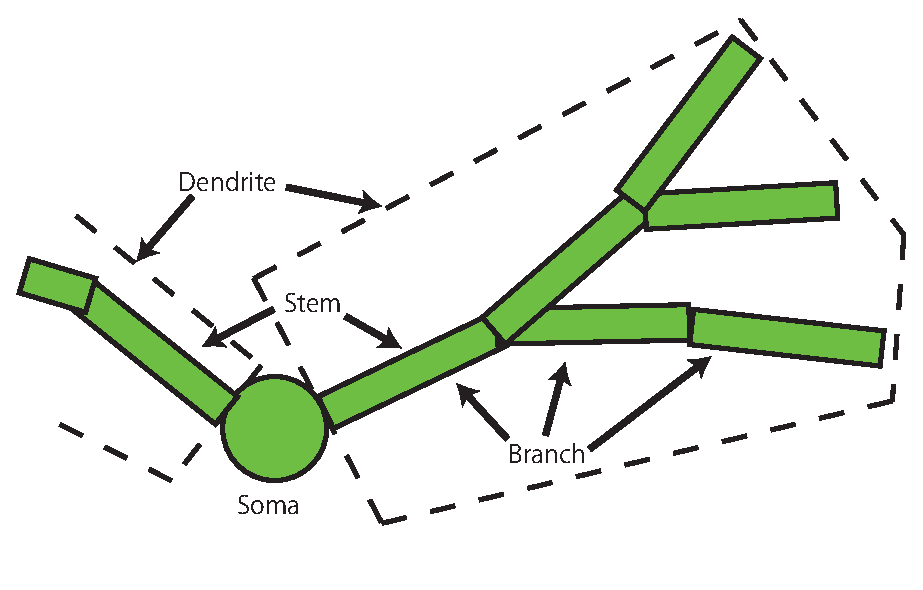
\includegraphics[width=10cm]{./Images_Method/neuron_morpho.eps}
       \caption{$B?@7P:YK&7ABV$K4X$9$kDj5A(B}
       \label{morpho}
     \end{figure}
   \subsection{$B<y>uFM5/7ABV@8@.<jK!$N4pK\35G0(B}
     $B<y>uFM5/7ABV@8@.<jK!$N4pK\$O(BL-system$B$G$"$k(B\cite{prusinkiewicz1990}.
     L-system$B$O(B, $B$"$k5-9f$N=89g$H$=$NCV$-49$(5,B'$+$iDj5A$5$l(B, $B=i4|>uBV$H$7$F$"$k5-9fNs$,M?$((B
     $B$i$l$k$H$=$N5-9fNs$r:F5/E*$KJQ49$7$F$$$/%7%9%F%`$G$"$k(B. L-system$B$NNc(B
     $B$r<($9(B\cite{torben2007evolving}. $B$^$:5-9f$N=89g(B$\{B,F,X,Y\}$$BDj5A$9(B
     $B$k(B. $B<!$K$=$NCV$-49$(5,B'$H$7$F(B
     \begin{align*}
       rules: \hspace{0.2cm} & F \to YF\\
       & X \to BX
     \end{align*}
     $B$rDj5A$9$k(B. $B=i4|>uBV$H$7$F5-9fNs(B$FX$$B$,M?$($i$l$?$H$9$k$H(B,
     L-system$B$OCV$-49$(5,B'$K=>$C$F$3$N5-9fNs$NCV$-49$($r:F5/E*$K9T$&(B. 2$B2s(B
     $BL\$NCV$-49$(=*N;$^$G$N5-9fNs$NJQ2=$O0J2<$N$h$&$K$J$k(B.
     \begin{align*}
       initial:\hspace{0.2cm} & FX \\
       1^{st} cycle:\hspace{0.2cm} & YFBX \\
       2^{nd} cycel:\hspace{0.2cm} & YYFBBX
     \end{align*}
     $B<y>uFM5/7ABV$N@8@.J}K!$H$7$F(B, $B;05\(B et al. $B$r;29M$K$9$k$H0J2<$N$h$&$J(BL-system$B$,9M$($i$l$k(B\cite{$B;05\?.IW(B1998$B0dEA%"%k%4%j%:%`$H:GE,2=(B}. 
     $B;HMQ$9$k5-9f$N=89g$H$7$F(B$\{S,B,T\}$$B$rDj5A$9$k(B.$BCV$-49$(5,B'$H$7$F(B
     \begin{align*}
       rules: \hspace{0.2cm}
       & S \to
       \begin{cases}
         T & \text{(Termination)}\\
         \begin{cases}
           <BS><BS> &\text{(Bifurcation)} \tag{$*$}\\
           BS &\text{(otherwise)}
         \end{cases} & \text{(otherwise)}
       \end{cases}\\
       & B \to B \\
       & T \to T
     \end{align*}
     $B$rDj5A$9$k(B. $B$3$N(BL-system$B$r7ABV@8@.(BL-system$B$H8F$V(B. 
     $B5-9f(B$S,B,T$$B$r<y>uFM5/$N9=B$$KCV$-49$($k$H(B, $B5-9f(BS$B$O<y>u(B
     $B9=B$$K$*$1$kL$@.D9$NE@$rI=$7(B, $B5-9f(BB$B$O(B$Branch$, $B5-9f(BT$B$O<y>uFM5/$N=*C<E@$KBP1~$9$k(B.
     $B$3$3$G(B, $<$\hspace{0.1cm}$>$$B$O<y>u9=B$$NJ,4t$rI=$7$F$$$k(B. $B$h$C$F(B,
     $B7ABV@8@.(BL-system$B$O(B1$B$D$NL$@.D9E@$r=i4|>uBV$H$7(B, $B$=$3$+$i<y>u9=B$$,@8@.$5$l$F$$$/2aDx$rI=8=$7$F$$$k(B. 
     $B5-9f(BS$B$NCV$-49$(5,B'(B($*$)$B$O7hDjE*$G$O$J$/(B, $B8e$K=R$Y$kJ,4t3NN($d=*C<3NN($K$h$C$F7hDj(B
     $B$5$l$k(B. 1$B$D$N<y>uFM5/$O=i4|>uBV(B$\{S\}$$B$+$i7ABV@8@.(BL-system$B$r3+;O$75-9fNs$,JQ(B
     $B2=$7$J$/$J$k$^$GCV$-49$($r9T$&$3$H$GF@$i$l$k(B. $B$^$?(B, $B:G$b:G=i$N5-9fCV$-49$($G$OI,$:(B$S \to BS$$B$N(B
     $BCV$-49$($,A*Br$5$l$k$h$&$K$9$k(B. \\
     $B:G=*E*$KF@$i$l$k5-9fNs$O5-9f(B$B$$B$H5-9f(B$T$$B$+$i$J$j(B, $B:G$b:8C<$K$"$k5-(B
     $B9f(B$B$$B$,(BStem$B$rI=$9(B. $B7ABV@8@.(BL-system$B$+$i0l$D$N<y>uFM5/$,@8@.$5$l$k2aDx$rNc<($9$k(B. $B$^$?(B
     $B?^(B\ref{fig:sample_L-system}$B$ONc$N(B$initial$, $3^{rd}cycle$, $finish$
     $B$r<y>u9=B$$H$7$FNc<($7$?$b$N$G$"$k(B. $B$3$3$G3F5-9f$NE:;z$OI}M%@hE*$K$D$1$i$l$F$$$/$3$H$K(B
     $BCm0U$5$l$?$$(B. % <- $B$3$3$I$&$J$s!)(B
     \begin{align*}
      initial:\hspace{0.2cm} & S_0 \\
      1^{st} cycle:\hspace{0.2cm} & B_1S_1 \\
      2^{nd} cycel:\hspace{0.2cm} & B_1<B_2S_2><B_3S_3> \\
      3^{rd} cycel:\hspace{0.2cm} & B_1<B_2B_4S_4><B_3T_1> \\
      4^{th} cycel:\hspace{0.2cm} & B_1<B_2B_4<B_5S_5><B_6S_6>><B_3T_1> \\
      \cdots \\
      finish:\hspace{0.2cm} & B_1<B_2B_4<B_5B_7B_{10}T_3><B_6<B_8T_2><B_9B_{11}T_4>>><B_3T_1> \\
     \end{align*}

     \begin{figure}[H]
      \centering
      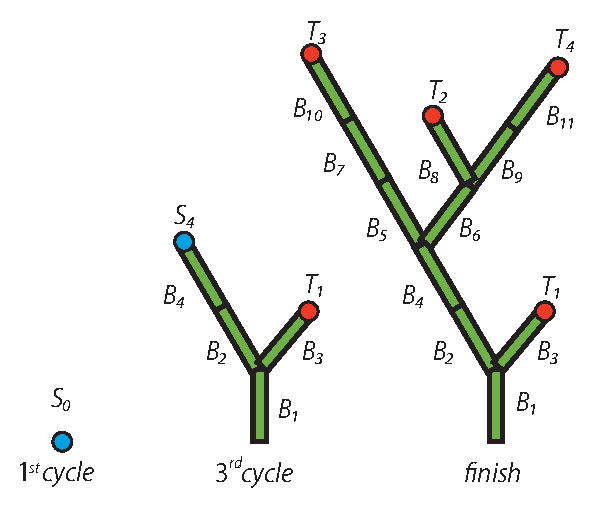
\includegraphics[width=10cm]{./Images_Method/L-system.eps}
      \caption{$B7ABV@8@.(BL-system$B$NE,MQNc(B}
      \label{fig:sample_L-system}
     \end{figure}

     $B$^$?(B, $B7ABV@8@.(BL-system$B$K$*$$$F5-9f(B$S_i$$B$NJ,4t$d?-D%$K$h$C$F(B
     $B?7$?$J5-9f(B$B_j$$B$,@8@.$5$l$k:]$K$O$=$l$KBP1~$7$?(B$Branch_j$$B$r0J2<$N(B\ref{makeBranch}$B@a(B
     $B$K<($9J}K!$G:n@.$9$k(B. 

   \subsection{$B%Q%i%a!<%?%;%C%H(B, $Branch$, $Dendrite$, $Neuron$$B$NDj5A(B}
     \subsubsection{$B%Q%i%a!<%?%;%C%H$NDj5A(B}
       1$B$D$N<y>uFM5/$O(B1$BAH$N%Q%i%a!<%?%;%C%H$+$i:n@.$5$l$k(B. $B>e=R$NDL$j(B, 1$B$D$N?@7P:YK&$O(B2$BK\$N<y>uFM5/(B
       $B$r;}$D$HDj5A$7$?$?$a(B, 1$B$D$N?@7P:YK&$O(B2$BAH$N%Q%i%a!<%?%;%C%H$+$i@8@.$5$l$k(B. 
       1$B$D$N%Q%i%a!<%?%;%C%H$K$O<y>uFM5/$N7ABV$r7hDj$9$k$?$a$N%Q%i%a!<%?$H<y>uFM5/>e$N(B
       $B%3%s%@%/%?%s%9J,I[$r7hDj$9$k$?$a$N%Q%i%a!<%?$,B8:_$9$k(B. $BA0<T$N%Q%i%a!<%?$r7ABV%Q%i%a!<%?(B, $B8e<T$N(B
       $B%Q%i%a!<%?$r%3%s%@%/%?%s%9%Q%i%a!<%?$H8F$V(B. 
       $BI=(B\ref{morpho_parameter}$B$O<y>uFM5/7ABV$r@8@.$9$k$?$a$K;HMQ$9$k7ABV%Q%i%a!<%?$G$"$k(B.

       \begin{table}[H]
         \caption{$B7ABV%Q%i%a!<%?(B}  % <- $B%Q%i%a!<%?$O:G8e$K$^$H$a$?J}$,$$$$$+$b(B
         \label{morpho_parameter}
         \begin{center}
           \begin{tabular}[H]{|c|l|l|} \hline
             \multicolumn{1}{|c}{No.} & \multicolumn{1}{|c}{$B%Q%i%a!<%?L>(B} & \multicolumn{1}{|c|}{$B@bL@(B} \\ \hline \hline
             1 &  \textit{Segment Length} [${\rm {\mu}m}$]& Stem$B$*$h$S(BBranch$B$ND9$5(B \\ \hline
             2 &  \textit{Stem diameter}  [${\rm {\mu}m}$]& Stem$B$ND>7B(B \\ \hline
             3 &  \textit{Stem elevation} [$^{\circ}$]& Stem$B$N6D3Q(B \\ \hline
             4 &  \textit{Stem rotation}  [$^{\circ}$]& Stem$B$N2sE>3Q(B \\ \hline
             5 &  \textit{Branch elevation $\mu$} [$^{\circ}$]& Branch$B$N6D3Q7hDj$KMQ$$$kJ?6QCM(B  \\ \hline
             6 &  \textit{Branch elevation $\sigma$} [$^{\circ}$] & Branch$B$N6D3Q7hDj$KMQ$$$kI8=`JP:9CM(B \\ \hline
             7 &  \textit{Branch rotation $\mu$}  [$^{\circ}$]& Branch$B$N2sE>3Q7hDj$KMQ$$$kJ?6QCM(B \\ \hline
             8 & \textit{Branch rotation $\sigma$} [$^{\circ}$] & Branch$B$N2sE>3Q7hDj$KMQ$$$kI8=`JP:9CM(B \\ \hline
             9 &  \textit{Bifurcation} $\alpha$ & $B<y>u9=B$$NJ,4tF3F~H=Dj$KMQ$$$k(B$k$$BCM(B \\ \hline
             10 & \textit{Bifurcation} $\beta$  & $B<y>u9=B$$NJ,4tF3F~H=Dj$KMQ$$$k(B$\theta$$BCM(B \\ \hline
             11 & \textit{Termination} $\alpha$ & $B<y>u9=B$$N=*C<E@F3F~H=Dj$KMQ$$$k(B$k$$BCM(B \\ \hline
             12 & \textit{Termination} $\beta$  & $B<y>u9=B$$N=*C<E@F3F~H=Dj$KMQ$$$k(B$\theta$$BCM(B \\ \hline
           \end{tabular}
         \end{center}
       \end{table}

       $B0J2<$K%3%s%@%/%?%s%9%Q%i%a!<%?$r<($9(B. $BK\8&5f$G$O<y>uFM5/>e$N%3%s%@%/%?%s%9J,I[$r7hDj$9$k:]$K(B
       $B;X?t4X?tE*$JJ,I[(B, $B$^$?$O%,%&%9J,I[$N$I$A$i$+$NJ,I[MM<0$rMQ$$$k(B. $B0J2<$G$O%3%s%@%/%?%s%9$r;X?t4X?tE*$K(B
       $BJ,I[$5$;$kJ,I[MM<0$r;X?t4X?tJ,I[$H8F$V(B. $B0lHLE*$J;X?tJ,I[$H$O0[$J$k$b$N$G$"$k$3$H$KCm0U$5$l$?$$(B. 
       $B<y>uFM5/>e$N%3%s%@%/%?%s%9$r;X?t4X?tJ,I[$5$;$k>l9g$O(B
       $BI=(B\ref{exp_parameter}$B$K<($5$l$k;X?t4X?tJ,I[%3%s%@%/%?%s%9%Q%i%a!<%?$r(B,
       $B%,%&%9J,I[$K=>$C$FJ,I[$5$;$k>l9g$K$O(B
       $BI=(B\ref{gausian_parameter}$B$K<($5$l$k%,%&%9J,I[%3%s%@%/%?%s%9%Q%i%a!<%?$r$=$l$>$lMQ$$$k(B.
       

       \begin{table}[H]
         \caption{$B;X?t4X?tJ,I[%3%s%@%/%?%s%9%Q%i%a!<%?(B}
         \label{exp_parameter}
         \begin{center}
           \begin{tabular}[H]{|c|l|l|} \hline
             \multicolumn{1}{|c}{No.} & \multicolumn{1}{|c}{$B%Q%i%a!<%?L>(B} & \multicolumn{1}{|c|}{$B@bL@(B} \\ \hline \hline
             13 & Ka \textit{Stem conductance} [${\rm S/cm^2}$]& Stem$B$N(BKa$B%3%s%@%/%?%s%9CM(B\\ \hline
             14 & Ka \textit{taper rate}  & Ka$B%3%s%@%/%?%s%9$NEAHBN((B \\ \hline
             15 & CaT \textit{Stem conductance} [${\rm S/cm^2}$]& Stem$B$N(BCaT$B%3%s%@%/%?%s%9CM(B \\ \hline
             16 & CaT \textit{taper rate}  & CaT$B%3%s%@%/%?%s%9$NEAHBN((B \\ \hline
           \end{tabular}
         \end{center}
       \end{table}

       \begin{table}[H]
         \caption{$B%,%&%9J,I[%3%s%@%/%?%s%9%Q%i%a!<%?(B}
         \label{gausian_parameter}
         \begin{center}
           \hspace*{-4em}
           \begin{tabular}[H]{|c|l|l|c|} \hline
             \multicolumn{1}{|c}{No.} & \multicolumn{1}{|c}{$B%Q%i%a!<%?L>(B} & \multicolumn{1}{|c|}{$B@bL@(B} \\ \hline \hline
             13 & Ka \textit{peak} [${\rm S/cm^2}$]&  Ka$B%3%s%@%/%?%s%9J,I[$N:GBgCM(B \\ \hline
             14 & Ka \textit{Gausian} $\mu$ & Ka$B%3%s%@%/%?%s%9J,I[$,=>$&%,%&%9J,I[$NJ?6QCM(B \\ \hline
             15 & Ka \textit{Gausian} $\sigma$ & Ka$B%3%s%@%/%?%s%9J,I[$,=>$&%,%&%9J,I[$NI8=`JP:9CM(B \\ \hline
             16 & CaT \textit{peak} [${\rm S/cm^2}$]&  CaT$B%3%s%@%/%?%s%9J,I[$N:GBgCM(B \\ \hline
             17 & CaT \textit{Gausian} $\mu$ & CaT$B%3%s%@%/%?%s%9J,I[$,=>$&%,%&%9J,I[$NJ?6QCM(B \\ \hline
             18 & CaT \textit{Gausian} $\sigma$& CaT$B%3%s%@%/%?%s%9J,I[$,=>$&%,%&%9J,I[$NI8=`JP:9CM(B \\ \hline
           \end{tabular}
         \end{center}
       \end{table}

       $B$h$C$F(B1$BAH$N%Q%i%a!<%?%;%C%H$O7ABV%Q%i%a!<%?$K%3%s%@%/%?%s%9%Q%i%a!<%?$r2C$($?(B16, $B$^$?$O(B18$B9`L\$G9=@.$5$l$F$$$k(B.
     \subsubsection{$Branch,Dendrite,Neuron$$B$NDj5A(B}
     $B$R$H$D$N(BBranch$B$OD9$5(B($length$), $BDlLL$ND>7B(B($diam$), $B6D3Q(B($elevation$),
     $B2sE>3Q(B($rotation$)$B$r7ABV$rI=8=$9$k%Q%i%a!<%?$H$7$F;}$D(B.
     $B$h$C$F(B, $B$"$k(B$Branch_i$$B$O(B4$B$D$N7ABV%Q%i%a!<%?$+$i$J$j(B,
       \begin{equation*}
         Branch_i = \{length_i, diam_i, elevation_i, rotation_i\}
       \end{equation*}
       $B$HI=$9$3$H$,$G$-$k(B. $B$^$?%$%s%G%C%/%9(B$i = 1$$B$N$H$-(B, $B$9$J$o$A(B$Branch_1$$B$O(BStem$B$G$"$k(B.
       $B$^$?(B$Dendrite$$B$O(B$Branch$$B$N=89g$G$"$j(B, 
       \begin{equation*}
         Dendrite_i = \{Branch_{i,1},Branch_{i,2},\dots,Branch_{i_{N_i}}\}
       \end{equation*}
       $B$^$?(B, 1$B$D$N?@7P:YK&(B($Neuron$)$B$O(B$Soma$$B$H(B2$B$D$N(B$Dendrite$$B$+$i$J$k(B. $B$h$C$F(B
       \begin{equation*}
         Neuron_i = \{Soma_i,Dendrite_{i,1},Dendrite_{i,2}\}
       \end{equation*}
       $B$H$J$k(B. 

 \subsection{$Branch$$B7ABV%Q%i%a!<%?7hDjJ}K!(B} \label{makeBranch}
   $B0J2<$K(B$Branch_i$$B$N%Q%i%a!<%?7hDjJ}K!$r=R$Y$k(B. $B$^$?(B, $B0J2<$N0lO"$N%Q%i%a!<%?7hDj<jK!$r(B
   $B4X?t(BmakeBranch($diam_{parent}$)$B$H$9$k(B. $B4X?t(BmakeBranch$B$O0z?t$H$7$F?F(B$Branch$$B$ND>7B(B$diam_{parent}$
   $B$r<h$j(B, $B?7$?$J(B$Branch$$B$rJV$94X?t$G$"$k(B. 
   \begin{enumerate}
    \item \textbf{$BD9$5(B({$length_i$})$B$N7hDj(B}\\
      $BD9$5(B$length_i$$B$O%Q%i%a!<%?%;%C%H$K$"$k(B
      \textit{Segment Length}$B$NCM$=$N$b$N$G$"$k(B. 
      \begin{equation}
        length_i = Segment\hspace{1mm} Length
      \end{equation}
    \item \textbf{$BD>7B(B($diam_i$)$B$N7hDj(B}\\
      {\textit Branch}$B$,J,4t(B(Bifurcation $ S \to <BS><BS>$)$B$K$h$C$F@8@.$5$l$k$+(B
      $B?-D%(B(Elongation $1 \to 21$)$B$K$h$C$F@8@.$5$l$k$+$K$h$C$F7hDjJ}K!$,0[$J$k(B. 
      \begin{itemize}
        \item{$BJ,4t(B(Bifurcation)$B$N>l9g(B} \\
          $B?F$H$J$k(B$Branch$$B$NB@$5(B($diam_{parent}$)$B$rMQ$$$F(B,
          $B%,%&%9J,I[(B($\mu = diam_{parent},\sigma=0.05$)
          $B$K=>$&Mp?t$r@8@.$7(B  , $B$=$NCM$r(B$diam_i$$B$H$9$k(B. $BJ?6Q(B$\mu$, $BI8=`JP:9(B$\sigma$$B$K=>$&(B
          $BMp?t$r(B1$B$D@8@.$9$k4X?t$r(BG($\mu,{\sigma}^2$)$B$H$9$k$H(B
          \begin{equation}
            diam_i = {\rm G}(diam_{parent},(0.05)^2)
          \end{equation}
        \item{$B?-D%(B(Elongation)$B$N>l9g(B} \\
          {\textit Branch}$B$,(BStem$B$G$"$k$+$I$&$+$K$h$C$F7hDjJ}K!$,0[$J$j(B, Stem$B$G$J$$>l9g$O(B
          $B?F$H$J$k(B$Branch$$B$ND>7B(B($diam_{parent}$)$B$r<B?tG\$7$?CM$rMQ$$$k(B
          \begin{equation}
            diam_i = 
            \begin{cases}
              Stem\hspace{1mm}diam & \text{(i = 1)}\\
              diam_{parent} \times taper\hspace{1mm}rate & \text{(otherwise)}\\
            \end{cases}\\
      \end{equation}
      $B$3$3$G(B, $taper\hspace{0.1cm}rate = 0.875$$B$G$"$j(B, $diam$$B$N8:?jN($rI=$9(B.
      \end{itemize}
    \item \textbf{$B6D3Q(B($elevation_i$)$B$N7hDj(B}\\
      {\textit diam}$B$HF1MM$K(BStem$B$G$"$k$+$I$&$+$G7hDjJ}K!$,0[$J$k(B. Stem$B$N>l9g$O7ABV%Q%i%a!<%?$N(B\textit{Stem elevation}$B$NCM$r(B
      $B$=$N$^$^MQ$$$k(B. Stem$B$G$J$$>l9g$OJ?6Q(B$\mu = Branch\hspace{1mm}elevation\hspace{1mm}\mu$,
      $BI8=`JP:9(B$\sigma = Branch\hspace{1mm}elevation\hspace{1mm}\sigma$$B$K=>$&%,%&%9J,I[$+$iMp?t$rH/@8$5$;(B, $B$=$NCM$r(B$elevation_i$$B$H$9$k(B.
      \begin{equation}
        elevation_i = 
        \begin{cases}
          Stem\hspace{1mm}elevation & \text{(i = 1)}\\
          {\rm G}(Branch\hspace{1mm}elevation\hspace{1mm}\mu,(Branch\hspace{1mm}elevation\hspace{1mm}\sigma)^2) & \text{(otherwise)}\\
       \end{cases}\\
      \end{equation}
    \item \textbf{$B2sE>3Q(B($rotation_i$)$B$N7hDj(B}\\
      $B6D3Q$N>l9g$HF1MM$K(B, $BJ?6Q(B$\mu = Branch\hspace{1mm}rotation\hspace{1mm}\mu$,
      $BI8=`JP:9(B$\sigma = Branch\hspace{1mm}rotation\hspace{1mm}\sigma$$B$K=>$&%,%&%9J,I[$+$iMp?t$rH/@8$5$;(B, $B$=$NCM$r(B$rotation_i$$B$H$9$k(B.
      \begin{equation}
        rotation_i = 
        \begin{cases}
          Stem\hspace{1mm}rotation & \text{(i = 1)}\\
          {\rm G}(Branch\hspace{1mm}rotation\hspace{1mm}\mu,(Branch\hspace{1mm}rotation\hspace{1mm}\sigma)^2) & \text{(otherwise)}\\
       \end{cases}\\
      \end{equation}
   \end{enumerate}

 \subsection{$B5-9f(BS$B$NCV$-49$(5,B'(B}
   $B7ABV@8@.(BL-system$B$K$*$1$k5-9f(B$B$$B$O(B$Branch$$B$KBP1~$7(B, $BJ8;zNs$O?^(B
   \ref{fig:sample_L-system}$B$K<($9$h$&$K<y>u9=B$$rI=8=$9$k(B.
   Stem, ($B_1$)$B$+$i<y>u9=B$$rC)$j(B, $BJ8;zNsCf$N$"$k5-9f(B$S_i$$B$K;j$k$^$G$KDL(B
   $B2a$9$k5-9f(B$B$$B$NE:$(;z$N=89g$r(B$J = \{1,2,\cdots,n\}$$B$H$9$k(B.
   $B$3$N$H$-(B$length_j\hspace{2mm}(j \in J)$$B$NOB$r(B${\rm path(S_i)}$$B$H$9$k(B.
   $B$9$J$o$A(B, $B5-9f(B$B_j$$B$rBP1~$9$k(B$Branch_j$$B$KCV$-49$(9=@.$5$l$k<y>u9=B$$r:,(B
   $B85$+$i5-9f(B$S_i$$B$N0LCV$^$GC)$C$?5wN%$G$"$k(B. 
   \begin{figure}[H]
     \centering
     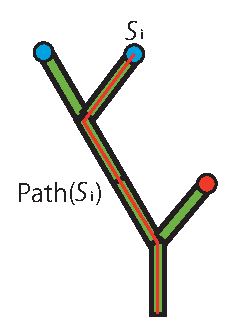
\includegraphics[width=5cm]{./Images_Method/path_S.eps}
     \caption{${\rm path}(S_i)$}
     \label{path(S_i)}
   \end{figure}
   $B0J2<$K5-9f(B$S_i$$B$NCV$-49$(5,B'(B($*$)$B$NA*BrJ}K!$H(B, $B$=$N:]$K9MN8$9$k%R%e!<(B
   $B%j%9%F%#%C%/%9$K$D$$$F<($9(B. $B$3$3$G(B$N_B$$B$r3FCV$-49$(%9%F%C%W$K$*$$$F$N(B
   $B5-9f(B$B$$B$NAm8D?t(B, $N_T$$B$r5-9f(B$T$$B$NAm8D?t$G$"$k$H$9$k(B. $B$^$?(B, $BCV$-49$($N(B
   $B=i4|>uBV$O(B$\{S_0\}$$B$HI=$9(B. 
   \begin{enumerate}
     \item \textbf{$BDd;_(B Termination $S_i \to T_{N_T + 1}$} \\
        $[0,1]$$B$NHO0O$G0lMMJ,I[$K=>$&Mp?t$r0l$D@8@.$7(B, $B$=$NCM$r(B$rand$$B$H$9$k(B.
        $BN_@Q%,%s%^J,I[(B\textit{Cumulative} $\gamma$($x,k,\theta$)$B$rMQ$$$F5-9f(B$S_i$$B$N?-D%Dd;_(B
        $B$NH=Dj$r9T$&(B. $B$=$N:](B, $BN_@Q%,%s%^J,I[$N%Q%i%a!<%?$H$7$F%Q%i%a!<%?%;%C%H$NCM$rMQ$$$k(B.
        \begin{equation}
	  {\rm Cumulative}\hspace{0.1cm}\gamma\hspace{0.05cm}({\rm path(S_i)},
          Termination\hspace{1mm}{\alpha},Termination\hspace{1mm}{\beta} ) > rand
        \end{equation}
        $B$H$J$k>l9g(B, $B?-D%Dd;_(B(Termination)$B$H$7(B$ S_i \to T_{N_T + 1}$$B$H$9$k(B.

      \item \textbf{$BJ,4t(B Bifurcation $ S_i \to <B_{N_B + 1}S_{N_B + 1}><B_{N_B + 2}S_{N_B + 2}>$} \\
        Termination$B$r9T$o$J$+$C$?>l9g$N$_(BBifurcation$B$NH=CG$r9T$&(B. 
        $[0,1]$$B$NHO0O$G0lMMJ,I[$+$iMp?t$r0l$D@8@.$7(B, $B$=$NCM$r(B$rand$$B$H$9$k(B.
        $B:GBgCM$,(B0.8$B$K$J$k$h$&$K<B?tG\$7$?%,%s%^J,I[(B
        Scaled $\gamma$($x,k,\theta$)$B$rMQ$rMQ$$$FJ,4t$NH=Dj$r9T$&(B. 
        $B$?$@$7%,%s%^J,I[$N%Q%i%a!<%?$H$7$F(B, $B%Q%i%a!<%?%;%C%H$NCM$rMQ$$$k(B. 
        \begin{equation}
	  {\rm Scaled}\hspace{0.1cm}\gamma\hspace{0.05cm}(path(S_i),
          Bifurcation\hspace{1mm}\alpha,Bifurcation\hspace{1mm}\beta) > rand
        \end{equation}
        $B$N$H$-J,4t(B(Bifurcation)$B$H$9$k(B. $B$9$J$o$A(B$Branch_i$$B$N(B$diam_i$$B$rMQ$$$F(B\\
        makeBranch($diam_i$)$B$+$i?7$?$K(B$Branch_{N_B + 1}$$B$H(B$Branch_{N_B + 2}$$B$r@8@.$9$k(B.
      \item \textbf{$B?-D%(B Elongation $S_i \to B_{N_B + 1}S_{N_B + 1}$} \\
        $B>e5-$N(B2$B>r7o$rK~$?$5$J$+$C$?>l9g(B, $B?-D%(B(Elongation)$B$H$9$k(B. 
        $B$9$J$o$A(B$Branch_i$$B$N(B$diam_i$$B$rMQ$$$F(BmakeBranch($diam_i$)$B$h$j(B, $B?7$?$K(B$Branch_{N_B + 1}$$B$r@8@.$9$k(B. 
    \end{enumerate}

   \subsubsection{$B7ABVE*%R%e!<%j%9%F%#%C%/(B}
    $B0J2<$N>r7o$K3:Ev$9$k>l9g$O6/@)E*$K?-D%Dd;_(B(Termination)$B$H$9$k(B. $B$3$l$O<y(B
    $B>uFM5/$H$7$FBEEv$J7ABV$rF@$k$?$a$KF3F~$9$k%R%e!<%j%9%F%#%C%/%9$G$"$k(B.    % <- $BBEEv$H$O(B?
    \begin{itemize}
      \item ${\rm path}(S_i) > 2000$$B$N$H$-(B
      \item $diam_{parent} \le Minimum\hspace{1mm}diameter$ $B$N$H$-(B\\ % <- $B%Q%i%a!<%?$r$"$H$G$^$H$a$?$[$&$,$$$$$+!)(B
       $B$^$?(B, $B$3$N>l9g(B, $B?F(B$Branch$$B$N(B$diam$$B$r(B$Minimum\hspace{1mm}diameter$
	    $B$K@_Dj$7D>$9(B.$B$3$3$G(B$Minimum\hspace{1mm}diameter = 0.15$[$\mu$m]$B$G$"$k(B. 
    \end{itemize}
    $B$3$l$i$N%R%e!<%j%9%F%#%C%/$O?@7P:YK&7ABV$r:n@.$9$k$?$a$K;HMQ$5$l$k$3$H$,B?$$(B\cite{burke1992parsimonious}. 

    \subsection{$Branch$$B$KBP$9$k;0<!85:BI8$N@_Dj(B}
     $length_i$, $elevation_i$, $rotation_i$$B$N>pJs$rMQ$$$F;0<!856u4V>e$G$N(B$Branch_i$$B$N:BI8>pJs$r(B
     $B@_Dj$9$k(B. $Branch_i$$B$N?-D%J}8~$O?F$H$J$k(BBranch$B$N8~$-$K$"$o$;$?Aj(B
     $BBPE*$J:BI8<4$rMQ$$$F9M$($k(B. $B6qBNE*$K$O0J2<$N$h$&$K$9$k(B. 
     \begin{itemize}
     \item \textbf{Stem$B$N3QEY@_Dj(B($i = 1$)}
       \begin{enumerate}
       \item $B6D3Q(B \\
	 $B6D3Q$r(B$elevation^{\circ}$$B$H$9$k(B. $B=i4|>uBV$H$7$F(BStem$B$O(B3$B<!856u4V(B
	 $B$N86E@$+$i(Bx$B<4$HF1$8J}8~$K?-$S$F$$$k$H$9$k(B. $B$3$N>uBV$+$i(BStem$B$r(B, z$B<4(B
	 $B$rCf?4$H$7$F1&$M$8$NJ}8~$K(B$elevation^{\circ}$$B2sE>$5$;$k(B.
	 $B$3$N:](By$B<4(B, x$B<4$bF1MM$K2sE>$r9T$$(B, $B$=$l$>$l(By'$B<4(B, x'$B<4$H(B
	 $B$9$k(B.$B$3$N>uBV$r?^(B\ref{elevation}$B$K<($9(B. 
       \item $B2sE>3Q(B \\
	 $B<!$K(B, $B2sE>3Q$r(B$rotation^{\circ}$$B$H$9$k(B. $B6D3Q$HF1MM$K(B,
	 Stem$B$r(By'$B<4$N1&$M$8$NJ}8~$K(B$rotation^{\circ}$$B2sE>$5$;$k(B. $B$^$?(B
	 x'$B<4(B, z$B<4$K$D$$$F$bF1MM$N2sE>$r9T$$(B, $B$=$l$>$l(Bx''$B<4(B, z'
	 $B<4$H$9$k(B. $B$3$N>uBV$r?^(B\ref{rotation}$B$K<($9(B. 
       \end{enumerate}
       \begin{figure}[h]
         \centering
         \begin{subfigure}{0.4\columnwidth}
           \centering
           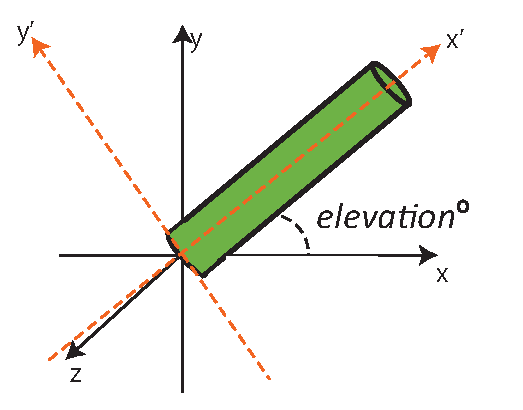
\includegraphics[width=\columnwidth]{./Images_Method/elevation.eps}
           \caption{elevation}
           \label{elevation}
         \end{subfigure}
         \begin{subfigure}{0.4\columnwidth}
           \centering
           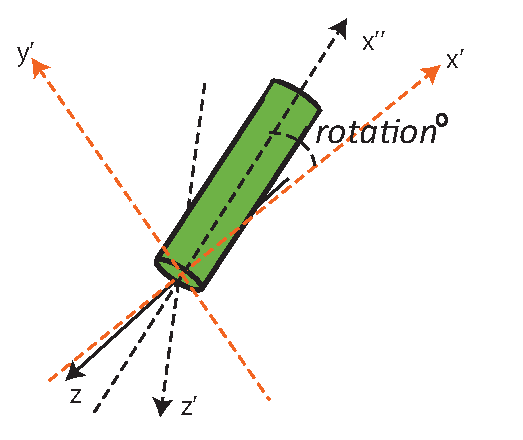
\includegraphics[width=\columnwidth]{./Images_Method/rotation.eps}
           \caption{rotation}
           \label{rotation}
         \end{subfigure}
         \caption{$B6D3Q(B, $B2sE>3Q$N@_Dj(B}
         \label{Branch_round}
       \end{figure}
     \item \textbf{Branch$B$N3QEY@_Dj(B} \\
       Stem$B$HF1MM$K9T$&(B. $B$?$@$7(B, $B$=$N(B$Branch$$B$N?F$H$J$k(B$Branch$$B$K$h$C(B
       $B$F2sE>$rM?$($?(Bx'',y',z'$B<4$rMQ$$$k(B. 
   \end{itemize}
     $B$3$l$i$N=hM}$N8e(B, $Dendrite$$BA4BN$r(B$Soma$$B$NI=LL$K@\$9$k$h$&$K(BStem$B$NJ}8~$K(B
     $BJ?9T0\F0$5$;$k(B. 

    \subsection{$B%7%J%W%F%#%C%/%>!<%s(B}
     3$B<!856u4V>e$N86E@$K(B$Soma$$B$rG[CV$7(B, $y$$B<4J}8~$N(B$170 < y < 190$$B$NHO0O$r(B % <- $B$3$NJU$N:BI8>pJs$rJQ?t$K$7$?$[$&$,$$$$$+$b(B
     Red$B%7%J%W%F%#%C%/%>!<%s(B, $y$$B<4J}8~$N(B$-170 > y > -190$$B$NHO0O$r(BBlue$B%7%J%W%F%#%C%/(B
     $B%>!<%s$HDj5A$9$k(B($B?^(B\ref{synaptic-zone}). $B%7%J%W%F%#%C%/%>!<%sFb$K(B$Branch$$B$,?/F~$7$?(B
     $B>l9g(B, $Branch$$B>e$K%7%J%W%9$rIUM?$9$k(B. $B6qBNE*$K$O2<5-(B
     \ref{synapse_setting}$B@a$K$F>\=R$9$k(B. 

 \section{$B?tM}%b%G%k(B}
   \subsection{$B:n@.$7$??@7P:YK&$N?tM}%b%G%k2=(B}
   $B7ABV@8@.(BL-system$B$K$h$C$FF@$i$l$?(B$Neuron$$B$r?tM}%b%G%k$KJQ49$9$k<jK!$r<($9(B. 
   1$B$D$N(B$Branch$$B$O:GBg(B5[$\mu$m]$B$NBg$-$5$KJ,3d$7$F(B, $B$=$l$>$l$KKlEE0L$r7W;;$9$k(B.
   $B$"$k<B?t(B$x$$B$KBP$7$F(B, $x$$B0J>e$N:G>.$N@0?t$rJV$94X?t$r(Bceiling($x$)$B$H$9$k(B.
   $B$3$N$H$-(B, $B$"$k(B$Branch_i$$B$rJ,3d$9$k8D?t(B$d_i$$B$O(B, $Branch_i$$B$ND9$5(B$length_i$
   $B$rMQ$$$F0J2<$N$h$&$KDj5A$9$k(B. 
   \begin{align}
     d_i &= 
     \begin{cases}
       {\rm ceiling}(\frac{length_i}{5}) & \text{(${\rm ceiling}(\frac{length_i}{5})$ is odd)}\\
       {\rm ceiling}(\frac{length_i}{5}) + 1 & \text{(${\rm ceiling}(\frac{length_i}{5})$ is even)}
     \end{cases}
   \end{align}
   $B$3$3$G(B$d_i$$B$r4q?t$H$9$k$N$O%7%_%e%l!<%7%g%s$K(BNEURON$B$rMQ$$$F$$$k$?$a$G$"$k(B.% <- $B$G$-$?$iM}M3$r=q$-$?$$(B
   $B$h$C$F(B$Branch_i$$B$O(B$\frac{length_i}{d_i}$$B$ND9$5$4$H$K(B1$B$D$N%3%s%Q!<%H%a%s%H$KJ,3d$5$l(B
   $Comp_{i,j}\hspace{1mm}(j = 1,2,\dots,d_i)$$B$H$J$k(B. 
   $B$^$?(B, $Soma$$B$O%3%s%Q!<%H%a%s%H$X$NJ,3d$O9T$o$J$$(B.
   \subsection{$B?@7P:YK&%b%G%k(B, $B%7%J%W%9%b%G%k(B}
     $B>e5-$NJ}K!$GJ,3d$5$l$?(B$Comp_{i,j}$$B$H(B$Soma$$B$O0J2<$N<0(B\ref{V_i}
     $B$rMQ$$$F$=$NKlEE0L$N5sF0$r%7%_%e%l!<%7%g%s$9$k(B. 
     $BC10l%3%s%Q!<%H%a%s%H$NKlEE0L(B($V_i$)$B$O0J2<$N<0$K$h$C$F7W;;$5$l$k(B.
     %g_leak$B$OJ?9UEE0L(B = -70$B$K$J$k$h$&$KD4@a$7$F$$$k(B
     \begin{equation}
       Cm\frac{dV}{dt} = - g_{leak}{\cdot}(V - E_{leak}) - I_{{\rm CaT}} - I_{{\rm Ka}}
       %$B$3$N(Bcm$B$O>.J8;z$+BgJ8;z$+(B?
       \label{V_i}
     \end{equation}
     $B%3%s%Q!<%H%a%s%H$NKl>e$K%7%J%W%9$,J,I[$7$F$$$k>l9g$O>e<0(B\ref{V_i}$B$N1&(B
     $BJU$K0J2<$N9`$r2C$($k(B.
     \begin{equation}
       (e^{-\frac{t}{{\tau}2}} - e^{-\frac{t}{{\tau}1}}) {\cdot} g_{syn} {\cdot} (V
       - E_{syn})
       \label{eq_syn}
     \end{equation}

     $B$^$?(B, $BB>$N%3%s%Q!<%H%a%s%H$,7k9g$7$F$$$k>l9g$O0J2<$N<0(B\ref{next_comp}$B$r(B
     $B<0(B\ref{V_i}$B$K2C$($k(B.
      $i$$BHVL\$N%3%s%Q!<%H%a%s%H$K(B$j$$BHVL\$N%3%s%Q!<%H%a%s%H$,7k9g$7$F$$$k$H$-(B,
     \begin{equation}
       g_{i,j} {\cdot}(V_j - V_i)
       \label{next_comp}
     \end{equation}
     $B$3$3$G(B$g_{i,j}$$B$O(B2$B$D$N%3%s%Q!<%H%a%s%H4V$N%3%s%@%/%?%s%9$rI=$7(B,
     $i$$BHVL\$N%3%s%Q!<%H%a%s%H$NH>7B$r(B${\alpha}_i$, $BD9$5$r(B$L_i$$B$H$9$k$H(B,
     $B0J2<$N<0$GI=$5$l$k(B.
     \begin{equation}
       g_{i,j} = \frac{{\alpha}_i{{\alpha}_j}^2}
       {Ra{\cdot}L_i(L_i{{\alpha}_j}^2 +  L_j{{\alpha}_i}^2)}
     \end{equation}
     
   \subsection{$B%$%*%s%A%c%M%k%b%G%k(B}
   $B<0(B\ref{V_i}$B$N%$%*%s%A%c%M%k%b%G%k(B$I_{CaT}$, $I_{Ka}$$B$O(B
   Migliore et al. $B$K<($5$l$k%$%*%s%A%c%M%k$N(B
     $B%b%G%k$r;HMQ$7$F$$$k(B\cite{migliore1995computer}. 
     \begin{itemize}
       \item $BEE0L0MB87?(BT$B7?(B${\rm Ca^{2+}}$$BEEN.(B
         \begin{align}
           I_{{\rm CaT}} &= g_{{\rm CaT}} {\cdot} ghk(V,cai,cao) \\                   
           g_{{\rm CaT}} &= \overline{g}_{{\rm CaT}} {\cdot} m^2 {\cdot} h  \\
           KTF &= \left(\frac{25.0}{293.15}\right) {\cdot} (T + 273.15) \\
           f &= \frac{KTF}{2} \\
           nu &= \frac{V}{f} \\
           ghk(V,cai,cao) &= -f {\cdot} \left(1.0 - \frac{C_i}{C_o} {\cdot} \exp(nu) \right) {\cdot} efun(nu) \\
           efun(z) &=
           \begin{cases}
             1 - \frac{z}{2} & (|z| < 10^{-4}) \\
             \frac{z}{(e^z - 1)} & (otherwise) \\
           \end{cases}
         \end{align}

         $B$^$?(B, CaT$B%3%s%@%/%?%s%9$N%2!<%HJQ?t(B($m$$B$*$h$S(B$h$)$B$N5sF0$O0J2<$NHyJ,J}Dx<0$K$h$C$FI=8=$5$l$k(B.
         
         \begin{align}
           {\tau}_{m}(V)\frac{dm}{dt} &= \frac{{\alpha}_m(V)}{{\alpha}_m(V) + {\beta}_m(V)} - m \\
           {\tau}_m(V) &= \frac{1}{{\alpha}_m(V) + {\beta}_m(V)} \\
           {\alpha}_m(V) &= 0.2{\cdot}\frac{-V + 19.26}{\exp(\frac{-V + 19.26}{10}) - 1} \\
           {\beta}_m(V) &= 0.009{\cdot}\exp(-\frac{V}{22.03})
         \end{align}

         \begin{align}
           {\tau}_{h}(V)\frac{dh}{dt} &= \frac{{\alpha}_h(V)}{{\alpha}_h(V) + {\beta}_h(V)} - h\\
           {\tau}_{h}(V) &= \frac{1}{{\alpha}_h(V) + {\beta}_h(V)} \\
           {\alpha}_h(V) &= 10^{-6}{\cdot}\exp(-\frac{V}{16.26}) \\
           {\beta}_h(V) &= \frac{1}{\exp(\frac{-V + 29.79}{10}) + 1}
         \end{align}

       \item A$B7?(BK$^+$$BEEN.(B
         \begin{align}
           I_{{\rm Ka}} &= g_{{\rm Ka}}{\cdot}(V - E_{{\rm K}}) \\
           g_{{\rm Ka}} &= \overline{g}_{{\rm Ka}}{\cdot}n{\cdot}l
         \end{align}
         $B$^$?(B, Ka$B%3%s%@%/%?%s%9$N%2!<%HJQ?t(B($n$$B$*$h$S(B$l$)$B$N5sF0$O0J2<$NHyJ,J}Dx<0$K$h$C$FI=8=$5$l$k(B.
         \begin{align}
           {\tau}_n(V)\frac{dn}{dt} &= \frac{1}{1 + {\alpha}_n(V)} - n \\
           {\tau}_n(V) &= \frac{{\beta}_n(V)}{Q_{10}{\cdot}{\alpha}_{0n}{\cdot}(1 + {\alpha}_n(V))} \\
           {\alpha}_n(V) &= {\exp}\left(\frac{10^{-3}{\cdot}{\zeta}_n{\cdot}(V - V_{n\frac{1}{2}}){\cdot}9.648{\cdot}10^4}
                                             {8.315{\cdot}(273.16 + T)} \right) \\
           {\beta}_n(V) &= {\exp}\left(\frac{10^{-3}{\cdot}{\zeta}_n{\cdot}gm_n{\cdot}(V - V_{n\frac{1}{2}}){\cdot}9.648{\cdot}10^4}
                                             {8.315{\cdot}(273.16 + T)} \right)
         \end{align}

         \begin{align}
           {\tau}_l(V)\frac{dl}{dt} &= \frac{1}{1 + {\alpha}_l(V)} - l \\
           {\tau}_l(V) &= \frac{{\beta}_l(V)}{Q_{10}{\cdot}{\alpha}_{0l}{\cdot}(1 + {\alpha}_l(V))} \\
           {\alpha}_l(V) &= {\exp}\left(\frac{10^{-3}{\cdot}{\zeta}_l{\cdot}(V - V_{l\frac{1}{2}}){\cdot}9.648{\cdot}10^4}
                                             {8.315{\cdot}(273.16 + T)} \right) \\
           {\beta}_l(V) &= {\exp}\left(\frac{10^{-3}{\cdot}{\zeta}_l{\cdot}gm_l{\cdot}(V - V_{l\frac{1}{2}}){\cdot}9.648{\cdot}10^4}
                                             {8.315{\cdot}(273.16 + T)} \right)
         \end{align}
     \end{itemize}

     $B$?$@$7(B
     \begin{align}
       Q_{10} &= 3^{(\frac{T - 30}{10})}
     \end{align}
     $B$G$"$k(B.
%
% gmn gml$B$O2?$J$N$+!)(B g_{mn}$B$J$N$+!)(B $BC10L$OL5$$$h$&$J$N$G!"(Bgmn$B$@$H;W$&(B
%
     $B?tM}%b%G%k$N%Q%i%a!<%?$r0J2<$NI=(B\ref{sim_param}$B$K<($9(B. % <- tau1 tau2$B$OJL$N%=!<%9%3!<%I$+$i$H$C$?$3$H$r=q$$$?$[$&$,$$$$(B

     \begin{table}[H]
       \caption{$B?tM}%b%G%k%Q%i%a!<%?(B}
       \label{sim_param}
       \centering
       \begin{subtable}{0.45\columnwidth}
         \centering
         \caption{$B?@7P:YK&%b%G%k%Q%i%a!<%?(B}
         \label{neuron_param}
         \begin{tabular}[h]{|c||c|} \hline
           \multicolumn{1}{|c||}{$B%Q%i%a!<%?L>(B} & \multicolumn{1}{c|}{$BCM(B} \\ \hline \hline
	   Simulation time [ms]& 50 \\\hline
	   $Ra$  [${\rm{\Omega}cm}$] & 100 \\ \hline
	   $Cm$  [${\rm{\mu}F/cm^2}$] & 0.8 \\ \hline
	   $V_{init}$ [mV]& -70\\ \hline
	   $g_{pas}$ [${\rm S/cm^2}$]& $2.5 \times 10^{-5}$\\ \hline
	   $E_{pas}$ [mV] & -70\\ \hline
           $g_{syn}$ [${\rm S/cm^2}$]& 0 \\ \hline
           $bv {\tau}_{1}$ [ms] & 0.5\\ \hline
	   ${\tau}_{2}$ [ms] & 2\\ \hline
         \end{tabular}
       \end{subtable}
       \begin{subtable}{0.45\columnwidth}
         \centering
         \caption{$B%$%*%s%A%c%M%k%b%G%k%Q%i%a!<%?(B}
         \label{cond_param}
         \begin{tabular}[h]{|c||c|} \hline
           \multicolumn{1}{|c||}{$B%Q%i%a!<%?L>(B} & \multicolumn{1}{c|}{$BCM(B} \\ \hline \hline
           $T$ [${\rm ^{\circ}C}$] & 37\\ \hline
           $E_{K}$ [mV] & -91\\ \hline
%           $\overline{g}_{CaT}$ [${\rm S/cm^2}$]& 0.003\\ \hline
%           $\overline{g}_{Ka}$ [${\rm S/cm^2}$]& 0.01\\ \hline
           ${\alpha}_{0n}$ [${\rm ms^{-1}}$]& 0.02\\ \hline
           ${\alpha}_{0l}$ [${\rm ms^{-1}}$]& 0.08\\ \hline
           ${\zeta}_n$ & -3\\ \hline
           ${\zeta}_l$ & 4\\ \hline
           $gm_n$ & 0.6\\ \hline
           $gm_l$ & 1\\ \hline
           $V_{n\frac{1}{2}}$ [mV]& -33.6\\ \hline
           $V_{l\frac{1}{2}}$ [mV]& -83\\ \hline
           $C_i$ [mM]& $5.0{\times}10^{-5}$\\ \hline
           $C_o$ [mM]& 2.0\\ \hline
         \end{tabular}
       \end{subtable}
     \end{table}

   \subsection{$B%3%s%Q!<%H%a%s%H>e$N%3%s%@%/%?%s%9J,I[@_Dj(B}
     $B:n@.$7$?(B$Comp_{i,j}$$B$N$=$l$>$l$K:GBg%3%s%@%/%?%s%9CM(B${\overline{g}_{\rm CaT}}_{i,j}$, ${\overline{g}_{\rm Ka}}_{i,j}$
     $B$r@_Dj$9$k(B. 
     $B<y>uFM5/>e$N%3%s%@%/%?%s%9J,I[$O;X?t4X?tJ,I[$H%,%&%9J,I[$N$I$A$i$+$r;HMQ$9$k(B.
     $B;X?t4X?tJ,I[$O3F(B$Branch$$B$N%3%s%@%/%?%s%9$NCM$r(B, $B?F(B$Branch$$B$N%3%s%@%/%?%s%9CM$N<B?tG\$H$7$F(B
     $B@_Dj$9$k(B\cite{torben2009systematic}. 
     $B%,%&%9J,I[$O(B$Comp$$B$4$H$K%3%s%@%/%?%s%9$rJQ2=$5$;$k(B.  $B$h$C$F;X?t4X?tJ,I[$N>l9g$h$j$b:Y$+$/%3%s%@%/%?%s%9(B
     $BJ,I[$r@_Dj$G$-$k(B. $B$^$?(B, $B<y>uFM5/$N$"$k0lIt$N$_$K9b$$%3%s%@%/%?%s%9J,I[$r;}$?$;$k$3$H$b2DG=$G$"$k(B. 
     $Soma$$B$KBP$7$F$O%3%s%@%/%?%s%9$rJ,I[$5$;$:(B,
     ${\overline{g}_{soma}}_{{\rm Ka}} = {{\overline{g}}_{soma}}_{\rm CaT} = 0$$B$H$7$?(B.
     $B$^$?(B, $B%3%s%@%/%?%s%9$N<h$j$&$k(BCaT$B%3%s%@%/%?%s%9$N:GBgCM$r(B\textit{Max} CaT, Ka$B$N:GBgCM$r(B\textit{Max} Ka$B$H$7(B,
     $B0J2<$NI=$K<($9(B.

     \begin{table}[H]
       \caption{$B:GBg%3%s%@%/%?%s%9NL(B}
       \label{sigma_M_init}
       \begin{center}
         \begin{tabular}[H]{c|c}
           \textit{Max} CaT [${\rm S/cm^2}$]& \textit{Max} Ka [${\rm S/cm^2}$] \\ \hline \hline
           0.0022 & 0.22 \\ 
         \end{tabular}
       \end{center}
     \end{table}

     $B0J2<$K(B$Comp_{i,j}$$B$KBP$9$k%3%s%@%/%?%s%9CM$N7hDjJ}K!$r=R$Y$k(B. 
     \begin{itemize}
     \item \textbf{$B;X?t4X?tJ,I[$N>l9g(B}\\
       $Branch$$BC10L$G%3%s%@%/%?%s%9$r@_Dj$9$k(B. $B$D$^$j$"$k(B$Branch_i$$B$+$iJ,3d$5$l$?%3%s%Q!<%H%a%s%H(B$Comp_{i,j}$$B$O(B
       $BA4$FF1$8%3%s%@%/%?%s%9CM$r;}$D(B. $Branch_i$$B$N%3%s%Q!<%H%a%s%H$N%3%s%@%/%?%s%9CM$r(B
       ${\overline{g}_{\rm CaT}}_{i}$, ${\overline{g}_{\rm Ka}}_{i}$$B$H$7(B,
       $B>e5-$N(B$diam$$B$HF1MM$K?F(B$Branch$$B$N;}$D%3%s%@%/%?%s%9(B$g_{parent_i}$$B$N<B?tG\$H$7$F7hDj$9$k(B\\
       \begin{align}
         {\overline{g}_{\rm CaT}}_{i,j} &= 
         \begin{cases}
           {\rm CaT}\hspace{1mm}Stem\hspace{1mm}conductance & \text{(i = 1)}\\
           {\overline{g}_{\rm CaT}}_{parent_i} \times {\rm CaT}\hspace{1mm}taper\hspace{1mm}rate & \text{(otherwise)}\\
         \end{cases} \\
         {\overline{g}_{\rm Ka}}_{i,j} &= 
          \begin{cases}
            {\rm Ka}\hspace{1mm}Stem\hspace{1mm}conductance & \text{(i = 1)}\\
            {\overline{g}_{\rm Ka}}_{parent_i} \times {\rm Ka}\hspace{1mm}taper\hspace{1mm}rate & \text{(otherwise)}
           \end{cases}
         \end{align}

       \item \textbf{$B%,%&%9J,I[$N>l9g(B}\\
         $B%3%s%Q!<%H%a%s%HC10L$G%3%s%@%/%?%s%9CM$r@_Dj$9$k(B. Stem$B$+$i(B$Comp_{i,j}$$B$^$G$N(B
         $length$$B$N9g7W$r(Bpath($Comp_{i,j}$)$B$H$9$k(B. 
         $B$^$?(B$Dendrite_i$$B$G$N:GBg$N(Bpath($Comp_{i,j'}$)$B$r(B
         max(Path($Comp_{i,j'}$))$B$H$9$k(B.
         $B$3$NFs$D$ND9$5$NHf$r(B\\
         path\hspace{1mm}ratio($Comp_{i,j}$)$B$H$7(B,
         \begin{equation}
         {\rm path}\hspace{1mm}{\rm ratio}(Comp_{i,j}) = \frac{Comp_{i,j}}{{\rm max(Path(}Comp_{i,j'}))}
         \end{equation}
         $B$H$9$k(B. 
         $B$3$N$H$-J?6QCM(B$\mu$, $BI8=`JP:9(B$\sigma$$B$N%,%&%9J,I[$+$i<B?t(B$x$$B$KBP$9$k3NN(L)EY$r(B
         $BJV$94X?t(BN($x,\mu,{\sigma}^2$)$B$rMQ$$$F(B
         \begin{align}
           {\rm Ka}\hspace{1mm}Gaus\hspace{1mm}Max &= {\rm N}({\rm Ka}\hspace{1mm}Gausian\hspace{1mm}\mu,{\rm Ka}\hspace{1mm}Gausian\hspace{1mm}\mu,({\rm Ka}\hspace{1mm}Gausian\hspace{1mm}\sigma)^2) \\
           {\rm CaT}\hspace{1mm}Gaus\hspace{1mm}Max &= {\rm N}({\rm CaT}\hspace{1mm}Gausian\hspace{1mm}\mu,{\rm CaT}\hspace{1mm}Gausian\hspace{1mm}\mu,({\rm CaT}\hspace{1mm}Gausian\hspace{1mm}\sigma)^2)
         \end{align}
         
         $B$H$7(B,
         
       \begin{align}
         {\overline{g}_{\rm Ka}}_{i,j} &=
         \frac{{\rm N}({\rm path}\hspace{1mm}{\rm ratio}(Comp_{i,j}),{\rm Ka}\hspace{1mm}Gausian\hspace{1mm}\mu,({\rm Ka}\hspace{1mm}Gausian\hspace{1mm}\sigma)^2)}
              {{\rm Ka}\hspace{1mm}Gaus\hspace{1mm}Max}
              \times {\rm Ka}\hspace{1mm}peak \\
         {\overline{g}_{\rm CaT}}_{i,j} &=
         \frac{{\rm N}({\rm path}\hspace{1mm}{\rm ratio}(Comp_{i,j}),{\rm CaT}\hspace{1mm}Gausian\hspace{1mm}\mu,({\rm CaT}\hspace{1mm}Gausian\hspace{1mm}\sigma)^2)}
              {{\rm CaT}\hspace{1mm}Gaus\hspace{1mm}Max}
              \times {\rm CaT}\hspace{1mm}peak
       \end{align}
     \end{itemize}
   $B$H$9$k(B.
   \subsection{$BC10l%3%s%Q!<%H%a%s%H$X$N%7%J%W%9$NIUM?(B} \label{synapse_setting}
     $B>e5-$N$h$&$KJ,3d$7$?(B$Comp_{i,j}$$B$,0lItJ,$G$b(B$170 < y < 190$$B$NNN0h$KF~$C$F$$$?>l9g(B,  % <- $B$3$NJU$N:BI8>pJs$rJQ?t$K$7$?$[$&$,$$$$$+$b(B
     Red$B%7%J%W%9$rIUM?$9$k(B. $B6qBNE*$K$O(B$Comp_{i,j}$$B$N(B
     $BKlEE0L$r<($9<0(B\ref{V_i}$B$N1&JU$K(B\ref{eq_syn}$B$r2C$($k(B. $B$^$?(B, y$B<4J}8~$N(B$-170 > y > -190$
     $B$KF~$C$F$$$?>l9g$O(BBlue$B%7%J%W%9$rIUM?$9$k(B.
     
 \section{$B0dEA%"%k%4%j%:%`(B}    % <- $B!V0dEA%"%k%4%j%:%`!W$H$$$&L>A0$O$I$&$J$N$+!)(B
   2$BAH$N%Q%i%a!<%?%;%C%H$r(B1$B$D$N8DBN$H$7$F(B200$B8DBN(B, $B@$Be?t(B500$B$G0dEA%"%k%4(B
   $B%j%:%`$rMQ$$$?%Q%i%a!<%?:GE,2=$r9T$C$?(B.  % <- $B0dEA%"%k%4%j%:%`$N%Q%i%a!<%?$b$I$3$+$GI=$K$^$H$a$?J}$,$$$$(B
   1$BAH$N%Q%i%a!<%?%;%C%H$r%Y%/%H%k(B$\overrightarrow{P}_i = \{p_{i,1},p_{i,2},\dots \}$
   $B$HI=$9$H(B, $B0l$D$N8DBN$O(B$u_i = \{\overrightarrow{P}_{i,1},\overrightarrow{P}_{i,2}\}$
   $B$HI=$5$l$k(B. 
   $B$^$?(B$\overrightarrow{P}_i$$B$+$i@8@.$5$l$k<y>uFM5/$r(B$Dendrite_i$$B$H$9$k(B. $B$h$C(B
   $B$F(B1$B$D$N8DBN(B$u_i$$B$+$i@8@.$5$l$k?@7P:YK&$O(B$Neuron_i = \{Dendrite_{i,1},Dendrite_{i,2}\}$
   $B$HI=$5$l$k(B.   
   $B$^$?(B, $B$"$k@$Be?t(B$g$$B$G$N(B$i$$BHVL\$N8DBN$r(B$u_{g,i}$$B$HI=$9(B. 
   $B$3$N0dEA%"%k%4%j%:%`$K$*$1$k0dEA;R$O8DBN(B$u_{g,i}$$B$N;}$D%Q%i%a!<%?%;%C%H(B$P_{g,i,1},P_{g,i,2}$
   $B$G$"$k(B. $B$^$?(B, $B@$Be?t(B$g = 1$$B$K$*$1$k8DBN$N%Q%i%a!<%?$N=i4|CM$O(B$P_{1,i,1},P_{1,i,2}$$B$H$b$K(B
   $B0J2<$NI=(B\ref{sigma_M_init}$B$K<($9CM$rMQ$$$k(B. $BI=(B\ref{sigma_M_init}$BCf$N5-9f(B
   U($\alpha,\beta$)$B$O(B$[\alpha,\beta]$$B$+$i0lMMMp?t$r(B1$B$DM?$($k4X?t$G$"$k$H$9$k(B. 
   $BK\8&5f$N0dEA%"%k%4%j%:%`$G$O(B, $B%(%j!<%HJ]B8(B, $B0lE@8r:5(B, $BFMA3JQ0[$rMQ$$$?(B.
   $B0J2<$K$=$N>\:Y$r=R$Y$k(B.
   \subsection{$B8DBNI>2A(B}
     $B3F@$Be(B$g$$B$G8DBN(B$u_{g,i}$$B$+$i?@7P:YK&7ABV(B$Neuron_{g,i}$$B$r@8@.$7$?8e(B,
     $B0J2<$N%7%_%e%l!<%7%g%s%W%m%H%3%k$r<B9T$9$k(B.
     \subsubsection{$B%7%_%e%l!<%7%g%s%W%m%H%3%k(B}
       $B$"$k8DBN(B$u_{g,i}$$B$+$i:n@.$5$l$?(B$Neuron_{g,i}$$B$KBP$7$F(B, $B0J2<$N%7%_%e%l!<%7%g%s$r9T$&(B.
       $B$^$?(BBlue$B%7%J%W%9$r3h@-2=$5$;$k;~9o$r(B$t_{Blue}$[ms],
       Red$B%7%J%W%9$r3h@-2=$5$;$k;~9o$r(B$t_{Red}$[ms]$B$H$9$k(B.
       $B%7%_%e%l!<%7%g%s;~4V$O(B50ms$B$G$"$k(B. $B$^$?(B, $Neuron_{g,i}$$B$N:YK&BN(B$Soma_{g,i}$$B$G4QB,$5$l$k:GBg$NKlEE0L>e>:NL$r(B
       $R$$B$H$9$k(B. $B%7%_%e%l!<%7%g%s$O0J2<$NI=(B\ref{synapse_time}$B$K<($5$l$k(B$t_{Blue}$, $t_{Red}$$B$NAH$_$rMQ$$$F(B,
       1$B$D$N(B$Neuron_{g,i}$$B$K$D$-7W(B4$B2s9T$o$l$k(B.
       $B%7%_%e%l!<%7%g%s$O(BNEURON$B%7%_%e%l!<%?$G9T$$(B, CVode$B%"%k%4%j%:%`$rMQ$$$?(B. % <- NEURON $B%7%_%e%l!<%?$K4X$7$F=q$$$?J}$,$$$$$+!)(B
       CVode$B%"%k%4%j%:%`$rMQ$$$k:]$N%(%i!<5vMFNL$O(B$10^{-5}$$B$K@_Dj$7$?(B. 
       
       \begin{table}[H]
         \caption{$B%7%J%W%93h@-2=;~9o(B}
         \label{synapse_time}
         \begin{center}
           \begin{tabular}[H]{|c||c|c||c|} \hline
               & $t_{Blue}$[ms] & $t_{Red}$[ms] & $R$ \\ \hline \hline
             1 & 5 & Not activated & $R_{Blue}$\\ \hline
             2 & Not activated & 5 & $R_{Red}$\\ \hline
             3 & 5 & ${\Delta}t$ + 5 & $R_{Blue \to Red}$\\ \hline
             4 & ${\Delta}t$ + 5 & 5 & $R_{Red \to Blue}$\\ \hline
           \end{tabular}
         \end{center}
       \end{table}

   \subsection{$BI>2ACM(B$E$$B$N7W;;(B}
     $B>e5-$N%7%_%e%l!<%7%g%s$N7k2L$r$b$H$K8DBN$NI>2A$r9T$&(B.
     $B8DBN$NI>2A$K$O(B, $B8DBN$N5!G=@-(B($B<0(B\ref{F})$B$N$[$+(B$Neuron$
     $B$NBN@Q(B, $BJ,I[$9$k%3%s%@%/%?%s%9$NNL$r9MN8$9$k(B. 
     $B$7$+$7(B, $B8DBN$K$h$C$F$O>e2<$N%7%J%W%F%#%C%/%>!<%s$K<y>uFM5/$r?-$P$;$:(B, 
     $B$=$b$=$b%7%_%e%l!<%7%g%s$r9T$&$3$H$,$G$-$J$$$b$N$,H/@8$9$k$3$H$b$"$k(B.
     $B$^$??@7P:YK&$r$h$j<BJ*$K6a$E$1$k$3$H$H(B, $BBEEv$J%7%_%e%l!<%7%g%s$r9T$&$3$H$r(B % <- $BBEEv$H$O!)(B
     $BL\E*$H$7$F$$$/$D$+$N%R%e!<%j%9%F%#%C%/%9$rF3F~$7$?(B. 
     $B$^$?(B, $B@$Be?t(B$g$, $BE:$(;z(B$i$$B$N8DBN$NI>2ACM(B$E$$B$r(B$E_{g,i}$$B$HI=5-$9$k(B
     $B0J2<$K8DBN$NI>2AJ}K!$r=R$Y$k(B. \\
     \begin{itemize}
       \item \textbf{$B7ABVE*%(%i!<(B}\\
         $B8DBN$+$i@8@.$7$?(B$Neuron$$B$,N>J}$N%7%J%W%F%#%C%/%>!<%s$K%7%J%W%9$r;}$?$:(B,
         $B%7%_%e%l!<%7%g%s$rA4$F9T$($J$$>l9g(B
         $Dendrite_{i,1}$$B$N(B$y$$B:BI8$N:GBgCM$r(Bmax($y_1$), $Dendrite_{i,2}$$B$N(B$y$$B:BI8$N(B
         $B:G>.CM$r(Bmin($y_2$)$B$H$7I>2ACM(B$E_{i,g}$$B$r(B
         \begin{equation}
           E_{g,i} = -{\rm max}\left(170 - {\rm max}(y_1),0\right) + {\rm min}\left(-170 - {\rm min}(y_2),0\right) - 100
           \label{Morpho_E}
         \end{equation}
         $B$H$9$k(B. 
       \item $B8DBN$+$i@8@.$7$?(B$Neuron$$B$,N>J}$N%7%J%W%F%#%C%/%>!<%s$K%7%J%W%9$r;}$A(B, $B>e5-(B4$B$D$N(B
         $B%7%_%e%l!<%7%g%s$rA4$F9T$C$?>l9g$O(B, $B$=$N@$Be$G$NAjBPE*$JI>2ACM$rM?$($k(B. $B$=$N$h$&$J8DBN(B
         $B$NE:$(;z$N=89g$r(B$S_g$$B$H$9$k(B. $B$3$3$G8DBN(B$u_{g,s}\hspace{1mm}(s \in S_g)$$B$K$D$$$F(B,
         $B$=$NCf$G$N:GBg$N(B$F$$BCM$r(Bmax$(F_g)$, $B$^$?8DBN(B$u_{g,s}$$B$+$i:n$i$l$?(B
         $B?@7P:YK&7ABV$r(B$Neuron_{g,s}$$B$H$7(B, $B$=$NCf$G:GBg$NBN@Q$r(B${Volume_{max}}_i$,
         CaT$B%3%s%@%/%?%s%9$N:GBg$N%3%s%@%/%?%s%9NL$r(B
         ${\rm CaT}\hspace{1mm}{{amount}_{max}}_g$, Ka$B%3%s%@%/%?%s%9$N:GBg$N(B
         $B%3%s%@%/%?%s%9NL$r(B${\rm Ka}\hspace{1mm}{{amount}_{max}}_g$$B$H$9$k(B.
         $B$3$3$G(B, $B%3%s%@%/%?%s%9NL$H$O$=$N(B$Neuron$$B$N3F%3%s%Q!<%H%a%s%H$NI=LL@Q$K%3%s%@%/%?%s%9(B
         $B$r$+$1$?CM$NAmNL$G$"$k(B. $B$3$N$H$-(B, $B$"$k8DBN(B$u_{g,i}$$B$NI>2ACM(B$E_{g,i}$$B$O0J2<$N$h$&$K7hDj$9$k(B.
         $B$^$:8DBN(B$u_{g,i}$$B$KJ,I[$9$k%3%s%@%/%?%s%9$NNL$rAjBPE*$KI=$9(B. $B$=$NCM$r(B
         $Conductance\hspace{1mm}ratio_{g,i}$$B$H$7(B, $B0J2<$N<0$K$h$C$F5a$a$k(B. 
         $B$3$3$G(B$N\hspace{1mm}Conductance$$B$O?@7P:YK&$KF3F~$7$F$$$k%$%*%s%A%c%M%k$N(B
         $B<oN`$N8D?t$G$"$k(B. % <-$B$J$s$+$U$o$C$H$7$F$k46$,$"$k(B
         
         \begin{equation}
           Conductance\hspace{1mm}ratio_{g,i} = \left(\frac{{\rm Ka}\hspace{1mm}amount_{g,i}}{{{\rm Ka}\hspace{1mm}amount_{max}}_{g}} +
           \frac{{\rm CaT}\hspace{1mm}amount_{g,i}}{{{\rm CaT}\hspace{1mm}amount_{max}}_{g}}\right) / N\hspace{1mm}Conductance
         \end{equation}

         $B$=$N8e(B, $B8DBN$NI>2ACM$r(B100$B$+$i$N8:E@J}<0$GM?$($k(B. 

         \begin{align}
           Function\hspace{1mm}Minus_{g,i} &= \left(1 - \frac{F_{g,i}}{{F_{max}}_g}\right) \times Function\hspace{1mm}ratio \\
           Morphology\hspace{1mm}Minus_{g,i} &= \frac{Volume_{g,i}}{{Volume_{max}}_g} \times Morphology\hspace{1mm}ratio \\
           Conductance\hspace{1mm}Minus_{g,i} &= \frac{Conductance\hspace{1mm}ratio_{g,i}}{{Conductance_{max}}_g} \times Conductance\hspace{1mm}ratio 
         \end{align}
         
         \begin{equation}
           E_{g,i} = 100 - (Function\hspace{1mm}Minus_{g,i} + Morphology\hspace{1mm}Minus_{g,i} + Conductance\hspace{1mm}Minus_{g,i})
           \label{E_equation}
         \end{equation}

     \end{itemize}

     $B$^$?(B, $B0J2<$N%R%e!<%j%9%F%#%C%/%9$K3:Ev$9$k8DBN$O(B, $B0J2<$N<0$K$h$C$FI>2A$9$k(B. %$B>e$N<0$H$N4XO"$O(B?
     \begin{itemize}
       \item \textbf{$B7ABVE*%R%e!<%j%9%F%#%C%/%9(B}\\
         $B0J2<$N>l9g$O%7%_%e%l!<%7%g%s$N7k2L$K0M$i$:(B, $B<0(B\ref{Morpho_E}$B$K$h$C$FI>2ACM(B
         $E_{g,i}$$B$rM?$($?(B. 
         \begin{itemize}
           \item $B?@7P:YK&A4BN$G(BStem$B$H(BBranch$B$N8D?t$,9g7W(B15$BL$K~$N>l9g(B
           \item $B?@7P:YK&A4BN$G<y>uFM5/$NJ,4t$,0l$D$b$J$$>l9g(B
         \end{itemize}
       \item \textbf{$B%7%_%e%l!<%7%g%s%R%e!<%j%9%F%#%C%/%9(B}\\
         $B0J2<$K<($5$l$k>l9g$O(B$\mu = -50$, $\sigma = 5$$B$N%,%&%9J,I[$+$iMp?t$r(B1$B$DH/@8$5$;(B,
         $B$=$NCM$rI>2ACM(B$E_{i,g}$$B$H$7$?(B.
         $B$3$l$O?@7P:YK&$G$NH/2P$d(B, $BKlEE0L$N?6F0$rM^@)$7(B, $B%7%_%e%l!<%7%g%s$N;~4VCf$K:GBg$N>e>:I}$,$H$l$k$h$&$K$9$k$?$a$G$"$k(B. 
         \begin{itemize}
           \item $ {R_{Blue}}_i < 2$$B$^$?$O(B$ {R_{Red}}_i < 2$$B$N$H$-(B
           \item ${R_{Blue}}_i > 25$$B$^$?$O(B${R_{Red}}_i > 25$$B$N$H$-(B
	   \item $B%7%_%e%l!<%7%g%s$N:G8e$N(B5$B%9%F%C%W$GKlEE0L$N>e>:$,5/$3$C$?$H$-(B
         \end{itemize}
         $B$3$N>r7o$KEv$F$O$^$C$?$H$-(B, $BI>2ACM(B$E_{g,i}$$B$O(B
         \begin{equation}
           E_{g,i} = {\rm G}(-50,5^2) % <- $B$3$N=q$-J}$O$"$C$F$k$N$+(B
           \label{penalty}
         \end{equation}
         $B$H$9$k(B. 
     \end{itemize}
     
   %% \begin{figure}[h] %$BI>2ACM$,AX>u$K$J$k$3$H$r8@$&$+!)(B
   %%   \centering
   %%   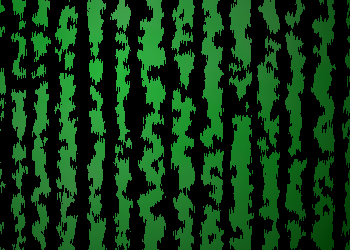
\includegraphics[width=5cm]{./Images_Method/temp.png} 
   %%   \caption{$BI>2ACM(B}
   %%   \label{Estimate}
     %% \end{figure}
     
   \subsection{$B%(%j!<%HJ]B8(B}
      $B@$Be(B$g$$B$K$*$$$F:GBg$NI>2ACM$r$H$C$?8DBN$O(B, $B$=$N$^$^(B$g + 1$$B@$Be$N(B1$B8DBN$K0z$-7Q$,$l$k(B.
      $B@$Be(B$g$$B$K$*$$$F$N8DBN$NE:$(;z$rI>2ACM$NBg$-$5=g$KJB$Y(B, $B=g0L(B$k$$B$N8DBN$NE:$(;z$r(B$r_k$$B$GI=$9(B
      $B$H$9$k(B. $B$3$N$H$-%(%j!<%HJ]B8$O(B
      
      \begin{equation}
       u_{g + 1,1} = u_{g,r_1}
      \end{equation}
      
      $B$HI=8=$G$-$k(B.
   \subsection{$B0lE@8r:5(B, $BFMA3JQ0[(B}
   %$B8r:5!"FMA3JQ0[$r5/$3$98DBN$N?t$OCf?46K8BDjM}E*$J9M$($G5a$a$i$l$k(B
     $B<!@$Be$N%(%j!<%H0J30$N8DBN$O0lE@8r:5$^$?$OFMA3JQ0[$N$I$A$i$+$N<jK!$K$h$C$F:n@.$5$l(B
     $B$k(B. $B0lE@8r:5$OI>2ACM>e0L(B$\mu$$B8D$N8DBN(B($u_{g,r_{1}},u_{g,r_{2}},\dots,u_{g,r_{\mu}}$)
     $B$r?F$H$7$F(B, $\lambda$$B8D$N;R8DBN$r@8@.$9$k(B. $B$3$3$G(B$\lambda = 50$$B$H$7$?(B. 
     $B$3$N(B$\lambda$$B8D$N;R8DBN$OI>2ACM2<0L(B$\lambda$$B8D$N8DBN$H8r49$5$l(B, $B<!@$Be$N8DBN$H$J$k(B.
     $BFMA3JQ0[$O;D$j$N(B$199 - \lambda$$B8D$N8DBN$KBP$7$FE,MQ$5$l$k(B.
     $B$3$3$G(B$\mu = 10$$B$G$"$k(B. $B$3$3$G(B$Parents_g =
     \{u_{g,r_{1}},u_{g,r_{2}},\dots,u_{g,r_{\mu}}\}$$B$H$7(B, Cross
     over($Parents$)$B$r0lE@8r:9$+$i<!@$Be8DBN$r0l$D:n@.$9$k4X?t$H$7(B,
     Mutation($u_{g,i}$)$B$r8DBN$KFMA3JQ0[$rM?$($k4X?t$G$"$k$H$9$k$H(B, $B<!@$(B
     $BBe8DBN(B$U_{g + 1}$$B$O(B
     \begin{equation}
      U_{g + 1} = \left(
       \begin{array}{c}
	u_{g,r_{1}}, \\
	{\rm Cross\hspace{1mm}over(Parent_g)}_{g + 1,2}, \\
	\dots \\
	{\rm Cross\hspace{1mm}over(Parent_g)}_{g + 1,\lambda + 1}, \\ % <- $B$3$l$O$o$+$j$K$/$$(B
	{\rm Mutation(u_{g,r_{1}})_{g + 1,\lambda + 2}}, \\
	\dots \\
	{\rm Mutation(u_{r_{g,199 - \lambda}})_{g + 1,200}}
       \end{array}
       \right)
     \end{equation}
     \begin{itemize}
       \item \textbf{$B0lE@8r:5(B Cross over}\\
	     $BI>2ACM>e0L$N(B$\mu$$B8DBN$+$i3NN(E*$K?F$r(B2$B8DBNA*Br$9$k(B. $B?F$rA*Br$9(B
	     $B$k:]$K$O0J2<$N<0(B\ref{Parent_P}$B$KDj5A$9$k3NN(J,I[$rMQ$$$F(B,
	     $B?F$NE:$(;z$r;XDj$9$k(B. $BI>2ACM$,(B$k$$BHVL\$N(B % <- $BI>2ACM$,Ii$N8DBN$J$I$bB8:_$7!"%k!<%l%C%HA*Br$J$I$,;H$($J$$$H$$$&$3$H$b=q$/(B
	     $B8DBN$,A*Br$5$l$k2DG=@-$r(B$P_k$$B$H$7(B, 
	     \begin{equation} % $BA*Br3NN($r1_%0%i%U$G?^<($9$k$+!)(B
	      P_k =  
	       \begin{cases}
		(\frac{1}{2})^k &  k < \mu\\
		(\frac{1}{2})^{k - 1} & otherwise
		 \end{cases}\\
	      \label{Parent_P}
	     \end{equation}
	     $B$H$9$k(B.
	     $B$J$*(B, $BF1$88DBN$,=EJ#$7$FA*Br$5$l$J$$$h$&$K$7$?(B. \\
	     $BA*Br$5$l$?(B2$B$D$N?F8DBN$NE:$(;z$r(B$x$, $y$$B$H$9$k(B. 
	     $B0lE@8r:5$O?F$N%Q%i%a!<%?%;%C%H(B$P_{g,i,1}$$BF1;N(B, $B%Q%i%a!<%?%;%C(B
	     $B%H(B$P_{g,i,2}$$BF1;N$G0J2<$N$h$&$K9T$&(B. %$B$J$<(BAB$B$rJ,$1$k$N$+$r=q$$$?J}$,$o$+$j$d$9$$(B
	     $B$3$l$O(B2$B$D$N(B$Dendrite_{i,1}$, $Dendrite_{i,2}$$B$r$=$l$>$lJL$N7OE}$H$7(B
	     $B$FE,1~$5$;$k$?$a$G$"$k(B.
         \begin{itemize}
           \item \textbf{$B8r:9E@$N7hDj(B} \\ %passive$B$N>l9g$O(BK,Ca$B%3%s%@%/%?%s%9$K4X$9$kItJ,$O8r:5$r9T$C$F$bL50UL#$@$C$?(B
             $B%Q%i%a!<%?%;%C%H$N9`L\?t$r(B$N_{Param}$$B$H$9$k(B. $B$3$N$H$-8r:9E@(B
		 \textit{Cross}$B$O(B$[N_{min},N_{max}]$$B$+$i(B
             $B0lMM$J3NN($G@0?t$r(B1$B$DJV$94X?t(BrandInt($N_{min}$,$N_{max}$)$B$rMQ$$$F(B
             \begin{equation}
               Cross = {\rm randInt}(1,N_{Param} - 1)
             \end{equation}
             $B$H$9$k(B. 
           \item \textbf{$B8r:5$N<B9T(B} \\
		 $B?7$?$J%Q%i%a!<%?%;%C%H$r:n@.$9$k(B. $B?7$?$J%Q%i%a!<%?%;%C%H$r(B
		 $\overrightarrow{P}_{new,i}$$B$H$9$k$H(B, $B?F$N%Q%i%a!<%?(B
		 $B%;%C%H(B$\overrightarrow{P_{x}}_{i}$,
		 $\overrightarrow{P_{y}}_{i}$$B$rMQ$$$F(B
		 \begin{equation}
		  \overrightarrow{P_{new}}_{i} = \{ {p_x}_{i,1}, {p_x}_{i,2},
		   \dots, {p_x}_{i,Cross}, {p_y}_{i,Cross + 1},
		   {p_y}_{i,Cross + 2}, \dots, {p_y}_{i,N_{Param}}\} %$BE:$(;z$,Hs>o$KHQ;((B
		 \end{equation}
         \end{itemize}
       \item \textbf{$BFMA3JQ0[(B Mutation}\\
        $B%Q%i%a!<%?%;%C%H$N3F9`L\$KBP$7$F(B0.65$B$N3NN($G%,%&%9J,I[(BG($\mu$,${{\sigma}_M}^2$)$B$K=>$&JQF0$rM?$($k(B. $B$9$J$o$A(B, $B$"$k%Q%i%a!<%?CM(B
         $p_i$$B$KBP$7$F(B, $B?7$7$$%Q%i%a!<%?CM(B${p'}_i$$B$O(B
         \begin{equation}
           {p'}_i = p_i + {\rm G}(p_i,{{\sigma}_M}^2)
           \label{Mutation}
         \end{equation}
         $B$H$J$k(B. $B$3$3$GMQ$$$k(B${\sigma}_M$$B$OFMA3JQ0[$rM?$($kBP>]$N%Q%i%a!<%?$K$h$C$F0J2<$NI=(B\ref{sigma_M}$B$K<($5$l$k(B
         $BCM$rMQ$$$k(B. $B$3$l$O%Q%i%a!<%?$K$h$C$FCM$N%l%s%8$,0[$J$k$?$a$G$"$k(B. 
         ${p'}_i$$B$,I=(B\ref{sigma_M}$B$K<($5$l$kCM0h$K<}$^$i$J$$>l9g$O:FEY<0(B\ref{Mutation}$B$rMQ$$$F(B
         ${p'}_i$$B$r<h$jD>$9(B. 
         \begin{table}[H]
           \caption{$BFMA3JQ0[$KMQ$$$kI8=`JP:9(B${\sigma}_M$$B$H3F%Q%i%a!<%?$N=i4|CM(B}
           \label{sigma_M_init}
           \begin{center}
	     \begin{tabular}[t]{|l||c|c|c|c|} \hline
           \multicolumn{1}{|c}{$B%Q%i%a!<%?L>(B} & \multicolumn{1}{|c|}{${\sigma}_M$} & \multicolumn{1}{c|}{$BCM0h(B} & \multicolumn{1}{c|}{$B=i4|CM(B}\\ \hline \hline
               \textit{Segment Length}            & 1                 & (0, $\infty$] & U(5,30)\\ \hline
	       \textit{Stem diameter}		  & 0.1		      & (0, 0.15]     & U(0.2,10)\\ \hline
	       \textit{Stem elevation}		  & 2		      & ($-{\infty}$, ${\infty}$) & U(-80,80)\\ \hline
	       \textit{Stem rotation}		  & 2		      & ($-{\infty}$, ${\infty}$) & U(0,360)\\ \hline
	       \textit{Branch elevation} $\mu$	  & 2		      & ($-{\infty}$, ${\infty}$) & U(0,8)\\ \hline
	       \textit{Branch rotation} $\mu$	  & 2		      & ($-{\infty}$, ${\infty}$) & U(0,8)\\ \hline
	       \textit{Branch elevation} $\sigma$ & 0.5		      & ($-{\infty}$, ${\infty}$) & 10 \\ \hline
	       \textit{Branch rotation} $\sigma$  & 0.5		      & ($-{\infty}$, ${\infty}$) & 10\\ \hline
	       \textit{Bifurcation} $\alpha$	  & 0.1		      & (1, ${\infty}$) & U(0,4) + 1\\ \hline
	       \textit{Termination} $\alpha$	  & 0.1		      & (1, ${\infty}$) & U(0,4) + 1\\ \hline
	       \textit{Bifurcation} $\beta$	  & 3		      & (1, ${\infty}$) & U(90,170)\\ \hline
	       \textit{Termination} $\beta$	  & 3		      & (1, ${\infty}$)  & U(5,50)\\ \hline
	       Ka \textit{Stem conductance}	  & 0.001	      & [0, \textit{Max} Ka] & U(0,0.08)\\ \hline
	       Ka \textit{peak}			  & 0.001     	      & [0, \textit{Max} Ka] & U(0,\textit{Max} Ka)\\ \hline
	       CaT \textit{Stem conductance}	  & 0.05$\cdot10^{-5}$ & [0, \textit{Max} CaT] & U(0,0.0001)\\ \hline
	       CaT \textit{peak}		  & 0.05$\cdot10^{-5}$ & [0, \textit{Max} CaT] & U(0,\textit{Max} CaT)\\ \hline
	       Ka \textit{taper rate}		  & 0.1		      & [0 , ${\infty}$) & U(0.85,1.15)\\ \hline
	       CaT \textit{taper rate}		  & 0.1    	      & [0 , ${\infty}$) & U(0.85,1.15)\\ \hline
	       Ka \textit{Gausian} $\mu$	  & 0.05	      & [0, 1] & U(0,1)\\ \hline
	       CaT \textit{Gausian} $\mu$	  & 0.05              & [0, 1] & U(0,1)\\ \hline
	       Ka \textit{Gausian} $\sigma$	  & 0.05	      & (0, ${\infty}$) & U($10^{-3}$,1.5)\\ \hline
	       CaT \textit{Gausian} $\sigma$	  & 0.05    	      & (0, ${\infty}$) & U($10^{-3},1.5$)\\ \hline
	     \end{tabular}					     
	   \end{center}						     
         \end{table}
     \end{itemize}

     %% \begin{table}[H]
       %%   \caption{$B0dEA%"%k%4%j%:%`%Q%i%a!<%?(B}
       %%   \label{GA-parameter}
       %%   \begin{center}
       %%     \begin{tabular}[H]{|c|l|l|c|} \hline
       %%       \multicolumn{1}{|c}{No.} & \multicolumn{1}{|c}{$B%Q%i%a!<%?L>(B} & \multicolumn{1}{|c|}{$B@bL@(B} & \multicolumn{1}{c|}{$BCM0h(B}\\ \hline \hline
       %%     \end{tabular}
       %%   \end{center}
       %% \end{table}

 \section{$B<B83<j=g(B}
   $B0J>e$NJ}K!$rMQ$$$F9T$C$?<B83$N@_Dj$K$D$$$F>\=R$9$k(B. 
   \subsection{$B<B83$K$*$1$kFHN)JQ?t(B}
     $BK\<B83$GA`:n$9$kFHN)JQ?t$K$D$$$F@bL@$9$k(B. $BFHN)JQ?t$O(BKa, CaT$B%$%*%s%A%c%M%k$NM-L5(B,
     2$B<oN`$N%7%J%W%9$r3h@-2=$5$;$k;~4V:9(B${\Delta}t$, $B<y>uFM5/>e$N%3%s%@%/%?%s%9J,I[MM<0(B,
     $B8DBNI>2A(B($B<0(B\ref{E_equation})$B$K$*$1$k%3%s%@%/%?%s%9$X$N9MN8$NM-L5$G$N(B4$B<oN`$G$"$k(B. 
     $B$=$l$>$l$NJQ?t$NAmEv$?$j$NAH$KBP$7$F>e5-$N0dEA%"%k%4%j%:%`$rMQ$$(B, $B:GE,$J(B$Neuron$$B$r5a$a$?(B.
     $B$^$?(B, $B$$$:$l$N;n9T$K$*$$$F$b;n9T?t$O(B10$B2s$H$7$?(B. 
     \begin{enumerate}
       \item \textbf{Ka, CaT$B%$%*%s%A%c%M%k$NM-L5(B} \\
         $BK\<B83$G$O?@7P:YK&$N%$%*%s%A%c%M%k$H$7$F(BKa$B%A%c%M%k(B, CaT$B%A%c%M%k$rMQ$$$k$,(B,
         $B$=$l$>$l$rMQ$$$k%Q%?!<%s$HMQ$$$J$$%Q%?!<%s$rMQ0U$7$?(B. $B$h$C$F%Q%?!<%s$H$7$F$O(B
         $BI=(B\ref{ion-channel_pattern}$B$N(B4$B$D$,$"$k(B. $BN>J}$N%$%*%s%A%c%M%k$r;HMQ$7$J$$%Q%?!<%s(B
         $B$r(BPassive$B$H8F$V(B. $B$J$*(B, $B%A%c%M%k$rMQ$$$J$$%Q%?!<%s(B
         $B$H$O(B, $B$=$N%$%*%s%A%c%M%k$N:GBg%3%s%@%/%?%s%9NL(B$\overline{g}$
         $B$r$9$Y$F$N%3%s%Q!<%H%a%s%H$K$*$$$F>o$K(B$\overline{g} = 0$$B$H$7$F$*$/$3$H$G$"$k(B. 
         \begin{table}[h]
           \caption{$B<y>uFM5/>e$N%$%*%s%A%c%M%k$N%Q%?!<%s(B}
           \label{ion-channel_pattern}
           \begin{center}
             \begin{tabular}[h]{|c||c|} \hline
                & $B%$%*%s%A%c%M%k(B \\ \hline \hline
               1 & $B$J$7(B(Passive) \\ \hline
               2 & Ka \\ \hline
               3 & CaT \\ \hline
               4 & Ka, CaT \\ \hline
             \end{tabular}
           \end{center}
         \end{table}

       \item \textbf{${\Delta}t$$B$N%Q%?!<%s(B} \\
         ${\Delta}t$$B$O(B5[ms]$B$+$i(B30[ms]$B$^$G(B5[ms]$B9o$_$K$7$?(B. $B$h$C$F;HMQ$7$?CM$O(B
         $BI=(B\ref{Delta_t_pattern}$B$N(B6$BDL$j$G$"$k(B.
         \begin{table}[H]
           \caption{${\Delta}t$$B$N%Q%?!<%s(B}
           \label{Delta_t_pattern}
           \begin{center}
             \begin{tabular}[h]{|c||c|} \hline
                & ${\Delta}t$[ms] \\ \hline \hline
               1 & 5 \\ \hline
               2 & 10 \\ \hline
               3 & 15 \\ \hline
               4 & 20 \\ \hline
               5 & 25 \\ \hline
               6 & 30 \\ \hline
             \end{tabular}
           \end{center}
         \end{table}
         
       \item \textbf{$B%3%s%@%/%?%s%9J,I[MM<0$N%Q%?!<%s(B} \\ % <- $B%3%s%@%/%?%s%9$H8@$C$?$j%A%c%M%k$H8@$C$?$j(B
         $B<y>uFM5/>e$N%3%s%@%/%?%s%9J,I[MM<0$OI=(B\ref{conductance_pattern}$B$K<($9$h$&$K(B
         $B;X?t4X?tJ,I[$+%,%&%9J,I[$N$I$A$i$+$rMQ$$$?(B.
         \begin{table}[H]
           \caption{$B%3%s%@%/%?%s%9J,I[MM<0$N%Q%?!<%s(B}
           \label{conductance_pattern}
           \begin{center}
             \begin{tabular}[h]{|c||c|} \hline
                & $B%3%s%@%/%?%s%9J,I[MM<0(B \\ \hline \hline
               1 & $B;X?t4X?tJ,I[(B \\ \hline
               2 & $B%,%&%9J,I[(B \\ \hline
             \end{tabular}
           \end{center}
         \end{table}
         
       \item \textbf{$B8DBNI>2A$K$*$1$k%3%s%@%/%?%s%9NL$NI>2A(B}
         $B8DBNI>2A$K%3%s%@%/%?%s%9$NNL$r9MN8$9$k>l9g$H(B, $B$7$J$$>l9g$G<0(B\ref{E_equation}$B$N(B
         $F$$BCM(B, $B:YK&7ABV(B, $B%3%s%@%/%?%s%9NL$KBP$9$k=E$_$NCM$K0J2<$NI=(B\ref{E_ratio}$B$NCM$r(B
         $BMQ$$$?(B.
         \begin{table}[H]
           \caption{$B8DBNI>2A$K;HMQ$9$k=E$_(B}
           \label{E_ratio}
           \begin{center}
             \begin{tabular}[h]{|c||c|c|c|} \hline
               &{\textit Function ratio}  & {\textit Morpho ratio} & {\textit Conductance ratio} \\ \hline \hline
               1, $B%3%s%@%/%?%s%9$N9MN8$J$7(B & 75 & 25 & 0\\ \hline
               2, $B%3%s%@%/%?%s%9$N9MN8$"$j(B & 75 & 20 & 5\\ \hline
             \end{tabular}
           \end{center}
         \end{table}
         $B%3%s%@%/%?%s%99MN8$J$7$N=E$_$NAH$O(B, Passive$B%?%$%W$N?@7P:YK&$N%7%_%e%l!<%7%g%s$K$F@h9T8&5f$N7k2L$r:F8=$9$k$3$H$,(B
         $B$G$-$?CM$NAH$G$"$k(B. {\textit Morpho ratio}$B$H(B{\rm Conductance ratio}$B$OBg$-$JCM$r$H$k$[$I(B, $Neuron$$B$NBg$-$5$H(B
         $B%3%s%@%/%?%s%9J,I[$N<+M3EY$rDc2<$5$;$k$H9M$($i$l(B, input-order detection$B$r<B8=$9$k>e$GIi$N8z2L$r;}$D$H(B
         $B9M$($i$l$k(B. $B$h$C$F%3%s%@%/%?%s%9$N9MN8$"$j$N>l9g$N(B{\textit Function ratio}$B$H(B,
         {\textit Morpho ratio}$B$H(B{\rm Conductance ratio}$B$NOB$NHf$O%3%s%@%/%?%s%99MN8$J$7$N>l9g$HEy$7$/$J$k$h$&$K$7$?(B. 
     \end{enumerate}     
   \subsection{$B2r@O9`L\(B}
     $B<B83$K$h$C$FF@$i$l$?:G=*@$Be$K$*$1$k:GNI8DBN$N7ABV(B, $B%3%s%@%/%?%s%9J,I[$K$D$$$F(B, $B0J2<$N9`L\$K$D$$$F2r@O$r9T$C$?(B. 
     \begin{itemize}
       \item \textbf{$B5!G=@-(B$F$$B$NCM(B}
       \item \textbf{$BD9$5(B[${\mu}m$]}\\
         $B?@7P:YK&$N;}$DA4$F$N(B$Branch$$B$N(B$length$$B$NOB(B
       \item \textbf{$BBN@Q(B[${\mu}m^3$]} \\
         $B?@7P:YK&$NA4$F$N(B$Branch$$B$NBN@Q$NOB(B

       \item \textbf{$B<y>uFM5/$ND>7B(B} \\
         $BK\8&5f$N7ABV@8@.$G$O(B, $B<y>uFM5/$N(B$Branch$$B$NB@$5$O(BStem$B$NCM$r$b$H$K7hDj$5$l$k(B. $B$=$N$?$a(BStem$B$ND>7B$r(B
         $B$=$N<y>uFM5/$NBeI=E*$JB@$5$H$7$FMQ$$$?(B. 

       \item \textbf{$B<y>uFM5/$NJ,4t?t(B} \\
         $B<y>uFM5/$K4^$^$l$kJ,4t$N8D?t$N9g7W(B

       \item \textbf{$B<y>uFM5/$N%7%J%W%9?t(B} \\
         $B<y>uFM5/$,$b$D%7%J%W%9$N8D?t$N9g7W(B

       \item \textbf{Ka$B%3%s%@%/%?%s%94^M-N((B} \\
         $B?@7P:YK&$N(BKa$B%3%s%@%/%?%s%94^M-N($O0J2<$N$h$&$KDj5A$9$k(B. 
         $B?@7P:YK&$N3F%3%s%Q!<%H%a%s%H(B$Comp_{i}$$B$K$D$$$F(B, $B$=$N(BKa$B%3%s%@%/%?%s%9$r(B${\overline{g}_{Ka}}_{i}$, 
         $BI=LL@Q$r(B$S_{i}$$B$H$9$k(B. $B?@7P:YK&$N%3%s%Q!<%H%a%s%H$N8D?t$r(B$N_C$$B$H$9$k(B. 
         $B?@7P:YK&$N(BKa$B%3%s%@%/%?%s%94^M-N((BKa \textit{ratio}$B$O(B, $B:GBg(BKa$B%3%s%@%/%?%s%9NL$G$"$k(B
         Max Ka$B$rMQ$$$F(B
         \begin{equation}
           {\rm Ka}\hspace{1mm}ratio = \frac{{\sum}^{N_C}_{i = 1}S_{i}\cdot{\overline{g}_{Ka}}_{i}}
           {{\sum}^{N_C}_{i = 1}S_{i}\cdot Max\hspace{1mm}{\rm Ka}}
         \end{equation}
         $B$H$9$k(B. 

       \item \textbf{CaT$B%3%s%@%/%?%s%94^M-N((B} \\
         $B?@7P:YK&$N(BCaT$B%3%s%@%/%?%s%94^M-N($O(B, Ka$B%3%s%@%/%?%s%9$N>l9g$HF1MM$KDj5A$9$k(B. 

        \item \textbf{$B%,%&%9J,I[$5$;$?%3%s%@%/%?%s%9$N%T!<%/0LCV(B} \\
          $B%3%s%@%/%?%s%9$r%,%&%9J,I[$K=>$C$FJ,I[$5$;$?>l9g$N%T!<%/$N0LCV(B($Gausian\hspace{1mm}\mu$)$B$r(B, 
          $B<y>uFM5/$ND9$5$r(B[0,1]$B$K@55,2=$7$?CM$GI=$9(B. $BCM$,(B1$B$K6a$$$[$I<y>uFM5/$N@hC<$K%T!<%/0LCV$,$"$k$3$H$rI=$9(B. 
          $B$7$+$7(B$peak$$B$,(B0$B$K6a$$>l9g$O(B$\mu$, $\sigma$$B$NCM$O0UL#$r$J$5$J$$(B. $B$=$N$?$a%T!<%/0LCV$N2r@O$G$O(B
          $B:GBg%3%s%@%/%?%s%9CM$N(B5\%$B0J>e$N(B$peak$$B$r$H$C$?>l9g$N(B$Gausian\hspace{1mm}\mu$$B$N$_$rMQ$$$?(B.
     \end{itemize}
     
